\chapter{Fase cuántica}
\thispagestyle{fancy}
\fancyhead[L]{\leftmark}

    \section{Cuantización del campo electromagnético}

        En la mecánica clásica, el estado de una partícula queda completamente determinado por su posición $q$ y su momento $p$. Estas variables evolucionan según las ecuaciones de Hamilton, y el espacio de fases $(q, p)$ contiene toda la información necesaria para predecir el comportamiento futuro del sistema. La estructura matemática subyacente está gobernada por los corchetes de Poisson, que para las variables canónicas satisfacen
        \begin{equation}
            \{q_i, p_j\} = \delta_{ij}, \quad \{q_i, q_j\} = \{p_i, p_j\} = 0.
        \end{equation}
        
        La primera cuantización consiste en promover estas variables clásicas a operadores que actúan sobre un espacio de Hilbert. La regla de correspondencia, establecida por Dirac \cite{Dirac1930}, reemplaza los corchetes de Poisson por conmutadores según
        \begin{equation}
            \{A, B\}_{\text{Poisson}} \longrightarrow \frac{1}{i\hbar}[\hat{A}, \hat{B}].
        \end{equation}
        
        De esta manera, las variables canónicas se convierten en operadores $\hat{q}$ y $\hat{p}$ que satisfacen las relaciones de conmutación canónicas
        \begin{equation}
            [\hat{p}_i, \hat{p}_j] = i\hbar\delta_{ij}, \quad [\hat{p}_i, \hat{p}_j] = [\hat{p}_i, \hat{p}_j] = 0.
        \end{equation}
        
        En este esquema, la función de onda $\psi(\mathbf{r}, t)$ describe la amplitud de probabilidad para encontrar la partícula en diferentes regiones del espacio. Un aspecto crucial es que el número de partículas permanece fijo: si comenzamos con una partícula, siempre tendremos una partícula. Esta limitación resulta ser fundamental cuando queremos describir fenómenos donde las partículas pueden crearse o destruirse, como ocurre con los fotones.

        La segunda cuantización representa un cambio de perspectiva radical. En lugar de tratar a las partículas como entidades fundamentales descritas por funciones de onda, elevamos los campos mismos a la categoría de operadores. Este procedimiento fue desarrollado por Fock \cite{Fock1932} y constituye la base matemática de la teoría cuántica de campos moderna.
    
        Consideremos un campo clásico $\phi(\mathbf{r}, t)$ que satisface alguna ecuación de movimiento. En la segunda cuantización, este campo se convierte en un operador $\hat{\phi}(\mathbf{r}, t)$ que actúa sobre un espacio de Hilbert especial llamado espacio de Fock. Este espacio se construye como la suma directa
        \begin{equation}
            \mathcal{F} = \bigoplus_{n=0}^{\infty} \mathcal{H}^{(n)} = \mathcal{H}^{(0)} \oplus \mathcal{H}^{(1)} \oplus \mathcal{H}^{(2)} \oplus \cdots
        \end{equation}
        donde $\mathcal{H}^{(0)} = \mathbb{C}$ corresponde al estado de vacío sin partículas, y $\mathcal{H}^{(n)}$ es el espacio de estados con exactamente $n$ partículas.
        
        La ventaja fundamental de este formalismo es que permite describir sistemas donde el número de partículas no está fijo. Los operadores de creación $\hat{a}^\dagger$ y aniquilación $\hat{a}$ actúan sobre el espacio de Fock conectando sectores con diferente número de partículas. Esta estructura resulta natural para describir la luz: los fotones se crean cuando un átomo emite radiación y se destruyen cuando la absorbe.
        
        La diferencia esencial entre ambos esquemas de cuantización puede resumirse así: en la primera cuantización, partimos de partículas clásicas y las hacemos cuánticas; en la segunda cuantización, partimos de campos clásicos y los hacemos cuánticos, obteniendo las partículas como excitaciones elementales del campo cuantizado.

        \begin{figure}[h]
            \centering    
            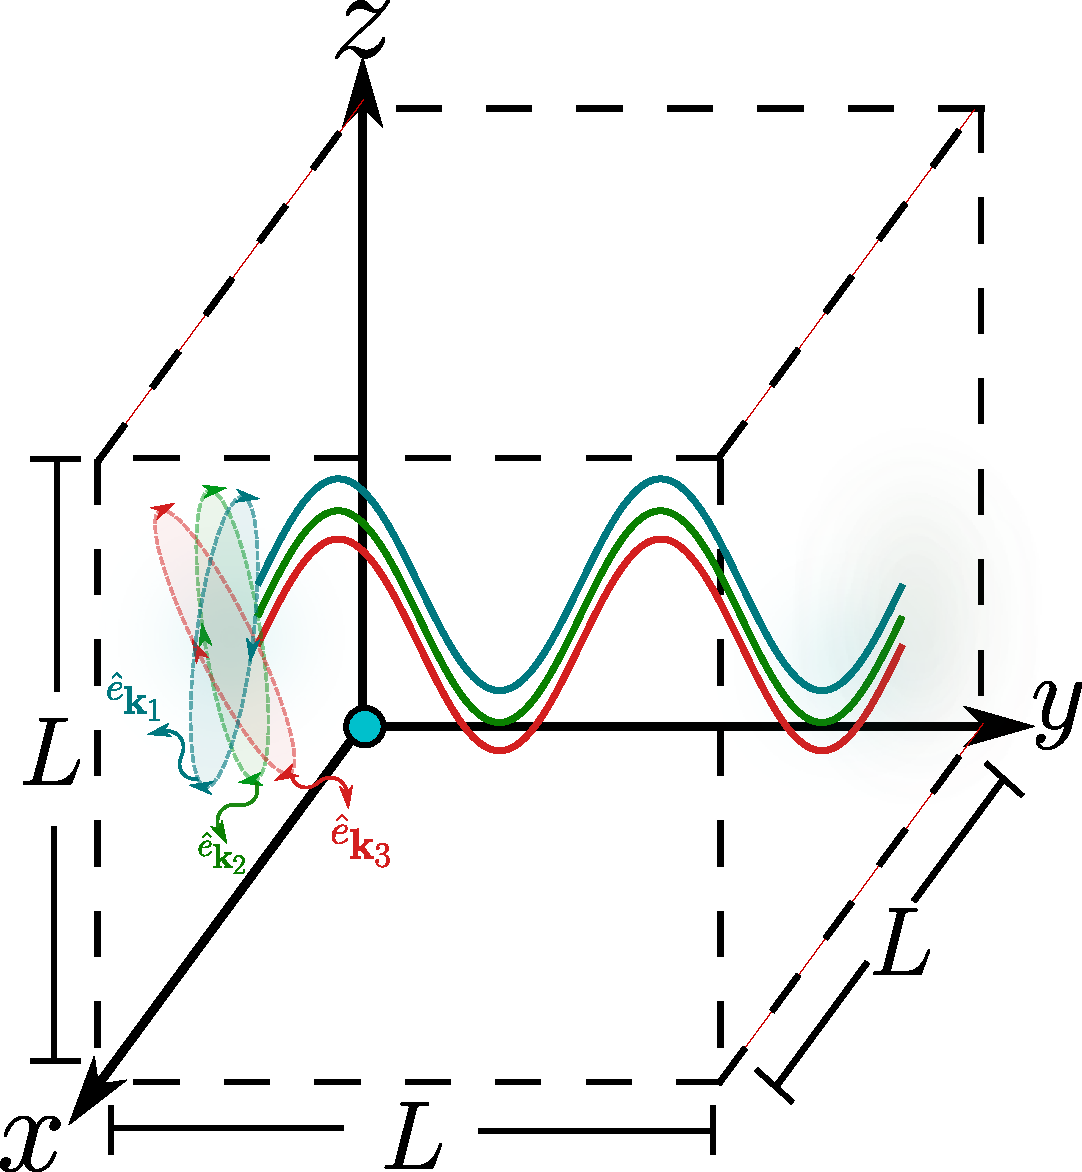
\includegraphics[width=0.5\textwidth]{Chapter3/Figures/CavidadL.pdf}
            \caption{Campo eléctrico en todos sus modos confinado en una cavidad con paredes conductoras perfectas}
            \label{fig:cavidad}
        \end{figure}

        Para desarrollar la teoría cuántica del campo electromagnético, resulta conveniente trabajar con un sistema confinado en una región finita del espacio (ver figura \ref{fig:cavidad}). La cavidad resonante proporciona el escenario ideal: un recinto cerrado con paredes perfectamente conductoras que imponen condiciones de frontera bien definidas. Este modelo, aunque idealizado, captura la física esencial y permite un tratamiento matemático riguroso que luego puede generalizarse al espacio libre mediante un proceso de límite apropiado.

        Consideremos una cavidad cúbica de lado $L$, sin cargas ni corrientes en su interior. Las ecuaciones de Maxwell en el vacío toman la forma \cite{Jackson1999}
        \begin{align}
            \nabla \cdot \mathbf{E} &= 0, \\
            \nabla \cdot \mathbf{B} &= 0, \\
            \nabla \times \mathbf{E} &= -\frac{\partial \mathbf{B}}{\partial t}, \\
            \nabla \times \mathbf{B} &= \frac{1}{c^2}\frac{\partial \mathbf{E}}{\partial t},
        \end{align}
        donde $c = 1/\sqrt{\mu_0 \epsilon_0}$ es la velocidad de la luz.
        
        Para resolver estas ecuaciones, introducimos el potencial vector $\mathbf{A}(\mathbf{r}, t)$ mediante la relación $\mathbf{B} = \nabla \times \mathbf{A}$, que satisface automáticamente la condición $\nabla \cdot \mathbf{B} = 0$. La ley de Faraday implica entonces que $\nabla \times (\mathbf{E} + \partial\mathbf{A}/\partial t) = 0$, de donde podemos escribir
        \begin{equation}
            \mathbf{E} = -\nabla \Phi - \frac{\partial \mathbf{A}}{\partial t}
        \end{equation}
        para algún potencial escalar $\Phi$.
        
        Los potenciales $\mathbf{A}$ y $\Phi$ no están determinados unívocamente por los campos físicos $\mathbf{E}$ y $\mathbf{B}$; existe la libertad de gauge. Adoptamos el gauge de Coulomb, definido por la condición
        \begin{equation}
            \nabla \cdot \mathbf{A} = 0.
        \end{equation}
        
        Esta elección tiene una consecuencia importante. En ausencia de cargas, la ecuación $\nabla \cdot \mathbf{E} = 0$ junto con el gauge de Coulomb implica $\nabla^2 \Phi = 0$. En una cavidad cerrada, la única solución compatible con condiciones de frontera finitas es $\Phi = 0$. Los campos quedan entonces expresados exclusivamente en términos del potencial vector transversal:
        \begin{equation}
            \mathbf{E} = -\frac{\partial \mathbf{A}}{\partial t}, \quad \mathbf{B} = \nabla \times \mathbf{A}.
        \end{equation}
        
        Sustituyendo en la ecuación de Ampère-Maxwell y utilizando la identidad $\nabla \times (\nabla \times \mathbf{A}) = \nabla(\nabla \cdot \mathbf{A}) - \nabla^2 \mathbf{A}$, obtenemos la ecuación de onda
        \begin{equation}
            \nabla^2 \mathbf{A} - \frac{1}{c^2}\frac{\partial^2 \mathbf{A}}{\partial t^2} = 0.
        \end{equation}

        Las paredes conductoras imponen que las componentes tangenciales del campo eléctrico se anulen en las fronteras. Buscamos soluciones mediante separación de variables, expandiendo el potencial vector en una serie de modos normales:
        \begin{equation}
            \mathbf{A}(\mathbf{r}, t) = \sum_{\mathbf{k},\lambda} q_{\mathbf{k},\lambda}(t) \, \mathbf{u}_{\mathbf{k},\lambda}(\mathbf{r}).
        \end{equation}
        
        Las funciones de modo $\mathbf{u}_{\mathbf{k},\lambda}(\mathbf{r})$ satisfacen la ecuación de Helmholtz $\nabla^2 \mathbf{u} + k^2 \mathbf{u} = 0$ junto con las condiciones de frontera. Para la cavidad cúbica, las soluciones involucran productos de funciones seno y coseno, y las condiciones de frontera cuantizan los componentes del vector de onda:
        \begin{equation}
            k_i = \frac{n_i \pi}{L}, \quad n_i = 0, 1, 2, 3, \ldots \quad (i = x, y, z).
        \end{equation}
        
        Cada vector $\mathbf{k}$ admite dos polarizaciones independientes, etiquetadas por $\lambda = 1, 2$. El gauge de Coulomb impone la condición de transversalidad $\mathbf{k} \cdot \hat{\boldsymbol{e}}_{\mathbf{k},\lambda} = 0$, de modo que los vectores de polarización son perpendiculares a la dirección de propagación. La frecuencia de cada modo está determinada por la relación de dispersión
        \begin{equation}
            \omega_{\mathbf{k}} = c\|\mathbf{k}\| = \frac{c\pi}{L}\sqrt{n_x^2 + n_y^2 + n_z^2}.
        \end{equation}
        
        Elegimos las funciones de modo normalizadas según
        \begin{equation}
            \int_V \mathbf{u}_{\mathbf{k},\lambda}(\mathbf{r}) \cdot \mathbf{u}_{\mathbf{k}',\lambda'}^*(\mathbf{r}) \, d^3r = \delta_{\mathbf{k},\mathbf{k}'}\delta_{\lambda,\lambda'},
        \end{equation}
        donde la integral se extiende sobre el volumen $V = L^3$ de la cavidad.
        
        Sustituyendo la expansión modal en la ecuación de onda y utilizando la ortogonalidad de las funciones de modo, encontramos que cada amplitud $q_{\mathbf{k},\lambda}(t)$ satisface
        \begin{equation}
            \ddot{q}_{\mathbf{k},\lambda}(t) + \omega_{\mathbf{k}}^2 q_{\mathbf{k},\lambda}(t) = 0.
        \end{equation}
        
        Esta es la ecuación de un oscilador armónico de frecuencia $\omega_{\mathbf{k}}$. Hemos llegado a un resultado fundamental: el campo electromagnético en una cavidad es dinámicamente equivalente a una colección infinita de osciladores armónicos independientes, uno por cada modo $(\mathbf{k}, \lambda)$.

        La energía total del campo electromagnético contenido en la cavidad es \cite{Jackson1999}
        \begin{equation}
            H = \frac{1}{2}\int_V \left(\epsilon_0 \|\mathbf{E}\|^2 + \frac{1}{\mu_0}\|\mathbf{B}\|^2\right) d^3r.
        \end{equation}
        
        Expresando los campos en términos del potencial vector y sustituyendo la expansión modal, el cálculo procede como sigue. Para el término eléctrico, usando $\mathbf{E} = -\partial\mathbf{A}/\partial t$:
        \begin{equation}
            \int_V \epsilon_0 \left\|\frac{\partial \mathbf{A}}{\partial t}\right\|^2 d^3r = \epsilon_0 \sum_{\mathbf{k},\lambda} |\dot{q}_{\mathbf{k},\lambda}|^2,
        \end{equation}
        donde hemos empleado la ortonormalidad de las funciones de modo.
        
        Para el término magnético, utilizamos que $\int_V \|\nabla \times \mathbf{u}_{\mathbf{k},\lambda}\|^2 d^3r = k^2 = \omega_{\mathbf{k}}^2/c^2$, lo cual conduce a
        \begin{equation}
            \int_V \frac{1}{\mu_0}\|\nabla \times \mathbf{A}\|^2 d^3r = \epsilon_0 \sum_{\mathbf{k},\lambda} \omega_{\mathbf{k}}^2 |q_{\mathbf{k},\lambda}|^2.
        \end{equation}
        
        Combinando ambas contribuciones, el Hamiltoniano total toma la forma
        \begin{equation}
            H = \frac{\epsilon_0}{2} \sum_{\mathbf{k},\lambda} \left(|\dot{q}_{\mathbf{k},\lambda}|^2 + \omega_{\mathbf{k}}^2 |q_{\mathbf{k},\lambda}|^2\right).
        \end{equation}
        
        Definiendo las variables canónicas $Q_{\mathbf{k},\lambda} = \sqrt{\epsilon_0} \, q_{\mathbf{k},\lambda}$ y $P_{\mathbf{k},\lambda} = \sqrt{\epsilon_0} \, \dot{q}_{\mathbf{k},\lambda}$, el Hamiltoniano adopta la forma estándar de una suma de osciladores armónicos:
        \begin{equation}
            H = \sum_{\mathbf{k},\lambda} \frac{1}{2}\left(P_{\mathbf{k},\lambda}^2 + \omega_{\mathbf{k}}^2 Q_{\mathbf{k},\lambda}^2\right).
        \end{equation}

        Habiendo establecido que el campo electromagnético clásico en una cavidad es equivalente a un conjunto de osciladores armónicos, procedemos ahora a su cuantización. El procedimiento sigue el esquema canónico: promovemos las variables dinámicas a operadores y reemplazamos los corchetes de Poisson por conmutadores.

        Las variables canónicas $Q_{\mathbf{k},\lambda}$ y $P_{\mathbf{k},\lambda}$ se convierten en operadores hermitianos $\hat{Q}_{\mathbf{k},\lambda}$ y $\hat{P}_{\mathbf{k},\lambda}$ que satisfacen las relaciones de conmutación
        \begin{equation}
            [\hat{Q}_{\mathbf{k},\lambda}, \hat{P}_{\mathbf{k}',\lambda'}] = i\hbar \delta_{\mathbf{k},\mathbf{k}'}\delta_{\lambda,\lambda'},
        \end{equation}
        mientras que los conmutadores entre operadores del mismo tipo se anulan:
        \begin{equation}
            [\hat{Q}_{\mathbf{k},\lambda}, \hat{Q}_{\mathbf{k}',\lambda'}] = [\hat{P}_{\mathbf{k},\lambda}, \hat{P}_{\mathbf{k}',\lambda'}] = 0.
        \end{equation}

        Para el oscilador armónico cuántico, resulta conveniente introducir combinaciones lineales de los operadores de posición y momento que simplifican la estructura algebraica. Definimos el operador de aniquilación
        \begin{equation}
            \hat{a}_{\mathbf{k},\lambda} = \sqrt{\frac{\omega_{\mathbf{k}}}{2\hbar}}\hat{Q}_{\mathbf{k},\lambda} + \frac{i}{\sqrt{2\hbar\omega_{\mathbf{k}}}}\hat{P}_{\mathbf{k},\lambda}
        \end{equation}
        y el operador de creación como su adjunto hermitiano
        \begin{equation}
            \hat{a}^\dagger_{\mathbf{k},\lambda} = \sqrt{\frac{\omega_{\mathbf{k}}}{2\hbar}}\hat{Q}_{\mathbf{k},\lambda} - \frac{i}{\sqrt{2\hbar\omega_{\mathbf{k}}}}\hat{P}_{\mathbf{k},\lambda}.
        \end{equation}
        
        Para determinar el álgebra de estos operadores, calculamos su conmutador. Usando las relaciones de conmutación canónicas:
        \begin{align}
            [\hat{a}_{\mathbf{k},\lambda}, \hat{a}^\dagger_{\mathbf{k}',\lambda'}] &= \frac{\omega_{\mathbf{k}}}{2\hbar}[\hat{Q}_{\mathbf{k},\lambda}, \hat{Q}_{\mathbf{k}',\lambda'}] - \frac{i}{2\hbar}\sqrt{\frac{\omega_{\mathbf{k}}}{\omega_{\mathbf{k}'}}}[\hat{Q}_{\mathbf{k},\lambda}, \hat{P}_{\mathbf{k}',\lambda'}] \nonumber \\
            &\quad + \frac{i}{2\hbar}\sqrt{\frac{\omega_{\mathbf{k}'}}{\omega_{\mathbf{k}}}}[\hat{P}_{\mathbf{k},\lambda}, \hat{Q}_{\mathbf{k}',\lambda'}] + \frac{1}{2\hbar\sqrt{\omega_{\mathbf{k}}\omega_{\mathbf{k}'}}}[\hat{P}_{\mathbf{k},\lambda}, \hat{P}_{\mathbf{k}',\lambda'}].
        \end{align}
        
        Los conmutadores $[\hat{Q}, \hat{Q}]$ y $[\hat{P}, \hat{P}]$ se anulan. Utilizando $[\hat{Q}_{\mathbf{k},\lambda}, \hat{P}_{\mathbf{k}',\lambda'}] = i\hbar\delta_{\mathbf{k},\mathbf{k}'}\delta_{\lambda,\lambda'}$ y $[\hat{P}_{\mathbf{k},\lambda}, \hat{Q}_{\mathbf{k}',\lambda'}] = -i\hbar\delta_{\mathbf{k},\mathbf{k}'}\delta_{\lambda,\lambda'}$, obtenemos
        \begin{equation}
            [\hat{a}_{\mathbf{k},\lambda}, \hat{a}^\dagger_{\mathbf{k}',\lambda'}] = \frac{1}{2}\delta_{\mathbf{k},\mathbf{k}'}\delta_{\lambda,\lambda'} + \frac{1}{2}\delta_{\mathbf{k},\mathbf{k}'}\delta_{\lambda,\lambda'} = \delta_{\mathbf{k},\mathbf{k}'}\delta_{\lambda,\lambda'}.
        \end{equation}
        
        Por construcción, también se tiene $[\hat{a}_{\mathbf{k},\lambda}, \hat{a}_{\mathbf{k}',\lambda'}] = [\hat{a}^\dagger_{\mathbf{k},\lambda}, \hat{a}^\dagger_{\mathbf{k}',\lambda'}] = 0$. Estas son las relaciones de conmutación bosónicas características de los fotones.
        
        Las relaciones pueden invertirse para expresar los operadores de posición y momento en términos de los operadores de escalera:
        \begin{align}
            \hat{Q}_{\mathbf{k},\lambda} &= \sqrt{\frac{\hbar}{2\omega_{\mathbf{k}}}}\left(\hat{a}_{\mathbf{k},\lambda} + \hat{a}^\dagger_{\mathbf{k},\lambda}\right), \\
            \hat{P}_{\mathbf{k},\lambda} &= i\sqrt{\frac{\hbar\omega_{\mathbf{k}}}{2}}\left(\hat{a}^\dagger_{\mathbf{k},\lambda} - \hat{a}_{\mathbf{k},\lambda}\right).
        \end{align}
 
        Estas relaciones expresan que modos diferentes son dinámicamente independientes; cada par $(\mathbf{k}, \lambda)$ constituye un grado de libertad cuántico separado.

        Los campos electromagnéticos se promueven a operadores sustituyendo las amplitudes clásicas por operadores cuánticos. El operador de campo eléctrico resulta

        \begin{equation}
            \hat{E}(\mathbf{r}, t) = i\sum_{\mathbf{k},\lambda} \sqrt{\frac{\hbar\omega_{\mathbf{k}}}{2\epsilon_0 V}} \left(\hat{a}_{\mathbf{k},\lambda} e^{-i\omega_{\mathbf{k}} t} - \hat{a}^\dagger_{\mathbf{k},\lambda} e^{i\omega_{\mathbf{k}} t}\right) \hat{\boldsymbol{\epsilon}}_{\mathbf{k},\lambda} f_{\mathbf{k}}(\mathbf{r}),
        \end{equation}
        donde $f_{\mathbf{k}}(\mathbf{r})$ representa la dependencia espacial del modo y $V = L^3$ es el volumen de la cavidad.
        
        Análogamente, el operador de campo magnético es
        \begin{equation}
            \hat{B}(\mathbf{r}, t) = i\sum_{\mathbf{k},\lambda} \sqrt{\frac{\hbar}{2\epsilon_0\omega_{\mathbf{k}} V}} \left(\hat{a}_{\mathbf{k},\lambda} e^{-i\omega_{\mathbf{k}} t} - \hat{a}^\dagger_{\mathbf{k},\lambda} e^{i\omega_{\mathbf{k}} t}\right) (\mathbf{k} \times \hat{\boldsymbol{\epsilon}}_{\mathbf{k},\lambda}) g_{\mathbf{k}}(\mathbf{r}).
        \end{equation}
        
        Ambos operadores son hermitianos, como corresponde a observables físicos. La combinación particular de operadores de creación y aniquilación, con sus respectivas fases temporales, garantiza que $\hat{E}^\dagger = \hat{E}$ y $\hat{B}^\dagger = \hat{B}$.


        \subsection{El Oscilador Armónico Cuántico de la radiación y los Estados de Fock}
            
            La estructura matemática que hemos desarrollado conduce naturalmente al oscilador armónico cuántico, uno de los sistemas más importantes de toda la física teórica. En el contexto de la óptica cuántica, las excitaciones del oscilador armónico corresponden a los fotones.

            Partimos del Hamiltoniano de un modo individual, $\hat{H}_{\mathbf{k},\lambda} = \frac{1}{2}(\hat{P}^2 + \omega^2\hat{Q}^2)$, donde omitimos los subíndices para simplificar la notación. Sustituyendo las expresiones de $\hat{Q}$ y $\hat{P}$ en términos de $\hat{a}$ y $\hat{a}^\dagger$:
            \begin{equation}
                \hat{H} = \frac{1}{2}\left[-\frac{\hbar\omega}{2}(\hat{a}^\dagger - \hat{a})^2 + \omega^2 \cdot \frac{\hbar}{2\omega}(\hat{a} + \hat{a}^\dagger)^2\right].
            \end{equation}
            
            Expandiendo los cuadrados y simplificando:
            \begin{align}
                (\hat{a}^\dagger - \hat{a})^2 &= \hat{a}^\dagger\hat{a}^\dagger - \hat{a}^\dagger\hat{a} - \hat{a}\hat{a}^\dagger + \hat{a}\hat{a}, \\
                (\hat{a} + \hat{a}^\dagger)^2 &= \hat{a}\hat{a} + \hat{a}\hat{a}^\dagger + \hat{a}^\dagger\hat{a} + \hat{a}^\dagger\hat{a}^\dagger.
            \end{align}
            
            Al restar estas expresiones, los términos $\hat{a}^\dagger\hat{a}^\dagger$ y $\hat{a}\hat{a}$ se cancelan, quedando
            \begin{equation}
                (\hat{a} + \hat{a}^\dagger)^2 - (\hat{a}^\dagger - \hat{a})^2 = 2(\hat{a}\hat{a}^\dagger + \hat{a}^\dagger\hat{a}).
            \end{equation}
            
            Usando la relación de conmutación $[\hat{a}, \hat{a}^\dagger] = 1$, podemos escribir $\hat{a}\hat{a}^\dagger = \hat{a}^\dagger\hat{a} + 1$, de donde $\hat{a}\hat{a}^\dagger + \hat{a}^\dagger\hat{a} = 2\hat{a}^\dagger\hat{a} + 1$. El Hamiltoniano resulta
            \begin{equation}
                \hat{H} = \hbar\omega\left(\hat{a}^\dagger\hat{a} + \frac{1}{2}\right).
            \end{equation}

            Definimos el operador número como
            \begin{equation}
                \hat{N} \equiv \hat{a}^\dagger\hat{a}.
            \end{equation}
            
            Este operador cuenta el número de excitaciones (fotones) en el modo. En términos del operador número, el Hamiltoniano de cada modo se escribe
            \begin{equation}
                \hat{H}_{\mathbf{k},\lambda} = \hbar\omega_{\mathbf{k}}\left(\hat{N}_{\mathbf{k},\lambda} + \frac{1}{2}\right),
            \end{equation}
            y el Hamiltoniano total del campo electromagnético es la suma sobre todos los modos:
            \begin{equation}
                \hat{H} = \sum_{\mathbf{k},\lambda} \hbar\omega_{\mathbf{k}}\left(\hat{N}_{\mathbf{k},\lambda} + \frac{1}{2}\right).
            \end{equation}
            
            Para entender la acción de los operadores de escalera, calculamos sus conmutadores con el operador número. Usando la identidad $[AB, C] = A[B, C] + [A, C]B$:
            \begin{align}
                [\hat{N}, \hat{a}] &= [\hat{a}^\dagger\hat{a}, \hat{a}] = \hat{a}^\dagger[\hat{a}, \hat{a}] + [\hat{a}^\dagger, \hat{a}]\hat{a} = 0 - \hat{a} = -\hat{a}, \\
                [\hat{N}, \hat{a}^\dagger] &= [\hat{a}^\dagger\hat{a}, \hat{a}^\dagger] = \hat{a}^\dagger[\hat{a}, \hat{a}^\dagger] + [\hat{a}^\dagger, \hat{a}^\dagger]\hat{a} = \hat{a}^\dagger \cdot 1 + 0 = \hat{a}^\dagger.
            \end{align}
            
            Estas relaciones tienen una interpretación inmediata. Si $\ket{n}$ es un autoestado del operador número con autovalor $n$, entonces
            \begin{equation}
                \hat{N}(\hat{a}\ket{n}) = \hat{a}(\hat{N} - 1)\ket{n} = (n-1)(\hat{a}\ket{n}),
            \end{equation}
            lo que muestra que $\hat{a}\ket{n}$ es autoestado con autovalor $n-1$. Análogamente, $\hat{a}^\dagger\ket{n}$ es autoestado con autovalor $n+1$. Por esto $\hat{a}$ se llama operador de aniquilación (reduce el número de excitaciones en uno) y $\hat{a}^\dagger$ se llama operador de creación (aumenta el número en uno).

            Para determinar los autovalores permitidos del operador número, observamos primero que $\hat{N}$ es semidefinido positivo:
            \begin{equation}
                \bra{\psi}\hat{N}\ket{\psi} = \bra{\psi}\hat{a}^\dagger\hat{a}\ket{\psi} = \|\hat{a}\ket{\psi}\|^2 \geq 0.
            \end{equation}
            
            Por tanto, todos los autovalores son no negativos. Si existiera un autovalor no entero $n = m + \epsilon$ con $0 < \epsilon < 1$ y $m$ entero, la aplicación sucesiva del operador de aniquilación produciría eventualmente un autovalor negativo, lo cual es imposible. Concluimos que los autovalores deben ser enteros no negativos: $n = 0, 1, 2, 3, \ldots$
            
            El estado con $n = 0$ es el estado de vacío $\ket{0}$, caracterizado por
            \begin{equation}
                \hat{a}\ket{0} = 0.
            \end{equation}
            
            Los estados con $n$ fotones, llamados estados de Fock o estados número, se construyen aplicando el operador de creación repetidamente:
            \begin{equation}
                \ket{n} = \frac{(\hat{a}^\dagger)^n}{\sqrt{n!}}\ket{0}.
            \end{equation}
            
            El factor $1/\sqrt{n!}$ asegura la normalización $\braket{n}{n} = 1$. Las acciones de los operadores de escalera sobre estos estados son
            \begin{align}
                \hat{a}\ket{n} &= \sqrt{n}\ket{n-1}, \\
                \hat{a}^\dagger\ket{n} &= \sqrt{n+1}\ket{n+1}.
            \end{align}
            
            La energía del estado con $n$ fotones en el modo $(\mathbf{k}, \lambda)$ es
            \begin{equation}
                E_n = \hbar\omega_{\mathbf{k}}\left(n + \frac{1}{2}\right).
            \end{equation}
            
            Los niveles de energía están igualmente espaciados, con separación $\hbar\omega_{\mathbf{k}}$ entre niveles consecutivos. Esta es precisamente la energía de un fotón de frecuencia $\omega_{\mathbf{k}}$, confirmando la interpretación corpuscular: cada excitación del campo corresponde a un fotón.

            El término $\frac{1}{2}\hbar\omega_{\mathbf{k}}$ representa la energía de punto cero del modo, presente incluso cuando no hay fotones. La energía total del vacío electromagnético es
            \begin{equation}
                E_{\text{vacío}} = \frac{1}{2}\sum_{\mathbf{k},\lambda} \hbar\omega_{\mathbf{k}}.
            \end{equation}
            
            Esta suma diverge, pues hay infinitos modos. En la práctica, esta contribución infinita se elimina mediante técnicas de renormalización o redefiniendo el Hamiltoniano con ordenamiento normal, donde todos los operadores de creación se colocan a la izquierda de los de aniquilación.
            
            Sin embargo, la energía del vacío tiene consecuencias físicas observables. El efecto Casimir \cite{Casimir1948}, la fuerza atractiva entre dos placas conductoras paralelas en el vacío, es una manifestación directa de las fluctuaciones cuánticas del campo electromagnético.

        \subsection{Los estados coherentes}

            Vamos a encontrar una familia de estados realmente importantes, primero encontrando cierta familia de estados especiales que a su vez son los autovalores del operador de aniquilación $\hat{a}$, sabemos que la mecánica cuántica debe producir los mismos resultados que la mecánica clásica en el caso límite en el que el oscilador armónico tiene una energía mucho mayor que la del cuanto de energía $\hbar \omega$.

            Por lo tanto, podemos plantear la siguiente pregunta: ¿es posible construir estados mecánicos cuánticos que conduzcan a predicciones físicas casi idénticas a las clásicas, al menos para un oscilador macroscópico? Veremos en este complemento que existen tales estados cuánticos: son superposiciones lineales coherentes de todos los estados. Los llamaremos \textit{estados cuasi-clásicos} o \textit{estados coherentes del oscilador armónico.}

            El problema que estamos considerando aquí es de gran interés general en la mecánica cuántica. Como bien se sabe en la mecánica cuántica muchos sistemas físicos pueden ser comparados con un oscilador armónico, al menos en una primera aproximación \cite{cohen1986quantum}. Para todos estos sistemas, es importante entender, en el marco de la mecánica cuántica, cómo pasar gradualmente del caso en el que los resultados dados por la aproximación clásica son suficientes al caso en el que los efectos cuánticos son preponderantes.

            La radiación electromagnética es un ejemplo muy importante de tal sistema. Dependiendo del experimento, revela su naturaleza mecánico cuántica o bien puede ser tratada clásicamente. Los estados coherentes de la radiación electromagnética fueron introducidos por Glauber y se utilizan actualmente en el campo de la óptica cuántica.

            Definimos los estados coherentes $\ket{\alpha}$ como los autoestados o estados propios del operador de aniquilación $\hat{a}$

            \begin{equation}
                \hat{a}\ket{\alpha} = \alpha\ket{\alpha}\;,
            \end{equation}

            podemos encontrar de muchas formas estos estados coherentes pero como conocemos bien los estados número $\ket{n}$ podemos encontrar los estados $\ket{\alpha}$ como una combinación lineal de los estados números pues estos conforman una base compelta y ortonormal, en este orden de ideas tenemos

            \begin{equation}
                \ket{\alpha} = \sum_m C_m \ket{m}\;,
            \end{equation}

            \begin{equation}
                \hat{\alpha}\ket{\alpha} = \sum_m C_m \sqrt{m}\ket{m-1} = \alpha \sum_n C_n \ket{n}\;,
            \end{equation}

            para el lado izquierdo de la ecuación vemos que se iguala al lado derecho cuando $m = n +1$ entonces tenemos la siguiente ecuación para los coeficientes de la expansión 
            
            \begin{equation}\label{eq:coefcnmahuno}
                C_{n+1}\sqrt{n + 1} = \alpha C_n \rightarrow C_{n+1} = \frac{\alpha}{\sqrt{n + 1}}C_n \;.
            \end{equation}

            La relación de recurrencia \ref{eq:coefcnmahuno} muestra un patrón en los coeficientes de la expansión, si evaluamos los primeros tres términos podemos ver dicho patrón:

            \begin{align*}
                & C_1 = \frac{\alpha}{\sqrt{1}}C_0\;,\\
                & C_2 = \frac{\alpha}{\sqrt{2}}C_1 = \frac{\alpha^2}{\sqrt{2*1}}C_0\;,\\
                & C_3 = \frac{\alpha}{\sqrt{3}}C_2 = \frac{\alpha^3}{\sqrt{3*2*1}}C_0\;.
            \end{align*}

            Es fácil ver que el enésimo coeficiente se puede expresar en términos del primer coeficiente de la siguiente manera,

            \begin{equation}
                C_n = \frac{\alpha^n}{\sqrt{n!}}C_0\;.
            \end{equation}

            Vemos que cuando $C_0$ está fijo, es decir, es constante, el enésimo coeficiente también lo será esto implica que el estado $\ket{\alpha}$ es único o a lo mucho varía en una constante de proporcionalidad, para determinar el coefeciente $C_0$ vamos a aprovecharnos de que el estado $\ket{\alpha}$ debe estar normalizado, entonces tenemos la siguiente ecuación 

            \begin{equation}
                \sum_n |C_n|^2 = 1\;,
            \end{equation}

            \begin{equation}
                \sum_n \frac{|\alpha^{2n}|}{n!}|C_0|^2 = 1\;,
            \end{equation}

            pero podemos darnos cuenta que la suma no es más que una expansión en series de Taylor de un exponencial,

            \begin{equation}
                |C_0|^2 e^{|\alpha|^2} = 1 \rightarrow C_0 = e^{-|\alpha|^2/2}\;.
            \end{equation}

            Ahora, podemos determinar los estados coherentes como:

            \begin{equation}\label{eq:CoherentStates}
                \ket{\alpha} = e^{-|\alpha|^2/2}\sum_n \frac{\alpha^n}{\sqrt{n}}\ket{n}\;.
            \end{equation}


            En este momento cabe preguntarse ¿qué está oscilando armónicamente? Si en el mundo macroscópico tenemos péndulos a pequeños ángulos o canicas oscilan en un pozo parabólico, en el contexto de la radiación ¿es el fotón el que está oscilando así? Para tratar de dar una solución a esto, primero desarrollemos la ecuación \ref{eq:CoherentStates} un poco más matemáticamente y luego veamos una representación gráfica tanto de los estados número como de los estados coherentes.

            Vamos a utilizar el teorema de desenlace \cite{sakurai1995modern}.

            \begin{theorem*}\label{teo:Desenlace}
                Sean $\hat{A}$ y $\hat{B}$ dos operadores, que no necesariamente conmutan, se cumple que la regla de exponenciación de la suma de $\hat{A}$ y $\hat{B}$ es:

                \begin{equation}
                    e^{\hat{A} + \hat{B}} = e^{\hat{A}}e^{\hat{B}}e^{-\frac{1}{2}[\hat{A},\hat{B}]} = e^{\hat{B}}e^{\hat{A}}e^{\frac{1}{2}[\hat{A},\hat{B}]}.
                \end{equation}

            \end{theorem*}

            Vamos a definir el operador de desplazamiento $\hat{\mathcal{D}}$ el cual jugará un rol importante en la interpretación física de los estados coherentes. El operador de desplazamiento es

            \begin{equation}
                \hat{\mathcal{D}}(\alpha) = e^{\alpha\hat{a}^{\dagger} - \alpha^*\hat{a}},
            \end{equation}

            y utilizando el teorema \ref{teo:Desenlace} entonces queda:

            \begin{equation}
                \hat{\mathcal{D}} = e^{-\frac{1}{2}|\alpha|^2}e^{\alpha \hat{a}^{\dagger}}e^{-\alpha^*\hat{a}}.
            \end{equation}

            Podemos expandir cada uno de los exponenciales, exceptuando el primero, en series de Taylor y haremos que actúe sobre el estado de vacío $\ket{0}$.

            \begin{equation}
                e^{-\alpha^*\hat{a}} \ket{0} = \sum_{k=0}^{\infty}\frac{(-\alpha^*\hat{a})^k}{k!}\ket{0} = \ket{0}\;,
            \end{equation}

            \begin{equation}
                e^{\alpha\hat{a}^{\dagger}}\ket{0} = \sum_{n=0}^{\infty}\frac{\alpha^n}{n!}(\hat{a}^{\dagger})^n\ket{0} = \sum_{n=0}^{\infty}\frac{\alpha^n}{n!}\ket{n}\;.
            \end{equation}

            En este orden de ideas, es fácil ver que aplicar el operador de desplazamiento sobre el estado de vacío $\ket{0}$ nos da origen a los estados coherentes $\ket{\alpha}$

            \begin{equation}
                \ket{\alpha} = \hat{\mathcal{D}}\ket{0}.
            \end{equation}

            Es decir, que los estados coherentes surgen al realizar desplazamientos de los estados de vacío, es decir, estados Gaussianos, los cuales oscilan como un oscilador armónico

    \section{Operadores de fase cuántica}
        La noción de fase es central en la física clásica de ondas. Para un campo electromagnético monocromático clásico de la forma $E(t) = E_0 \cos(\omega t + \phi)$, la amplitud $E_0$ y la fase $\phi$ son cantidades perfectamente definidas que admiten medición simultánea con precisión arbitraria. En el régimen cuántico, sin embargo, la situación es cualitativamente diferente: la amplitud del campo está relacionada con el número de fotones y la fase constituye, en cierto sentido, la variable canónicamente conjugada al número de excitaciones. Como veremos, intentar definir un operador de fase hermitiano que sea canónicamente conjugado al operador número conduce a contradicciones matemáticas profundas que la comunidad de óptica cuántica tardó décadas en comprender plenamente \cite{Barnett1989,Lynch1995,Perinova1998}.
    
        El problema puede enunciarse de manera precisa desde el principio. Definimos el operador número $\hat{N} = \hat{a}^{\dagger}\hat{a}$, con autovalores $n \in \{0, 1, 2, \ldots\}$ y autoestados $|n\rangle$ (estados de Fock). Si existiera un operador de fase hermitiano $\hat{\phi}$ que fuera canónicamente conjugado a $\hat{N}$, debería satisfacer
        \begin{equation}
            [\hat{N}, \hat{\phi}] = i,
            \label{eq:conmutador_n_phi}
        \end{equation}
        en perfecta analogía con el par posición--momento $[\hat{x}, \hat{p}] = i\hbar$. De esta relación se esperarían consecuencias físicas precisas: una relación de incertidumbre $\Delta n \cdot \Delta\phi \geq 1/2$, autoestados de fase bien definidos, y un operador unitario $e^{i\hat{\phi}}$ que actuara como operador de desplazamiento en número. Como demostraremos, ninguna de estas propiedades puede satisfacerse simultáneamente, y el motivo radica en la naturaleza semiboundada del espectro del operador número.
        
        Las dificultades fundamentales del problema de la fase cuántica son de dos tipos. El primero es algebraico: el espectro del operador número está acotado inferiormente por cero, lo que impide la existencia de un operador hermitiano con espectro en $[0, 2\pi)$ que satisfaga \eqref{eq:conmutador_n_phi} en todo el espacio de Fock. El segundo es físico: para estados con pocos fotones, la distinción entre diferentes propuestas de operador de fase es apreciable y experimentalmente relevante, por lo que la elección del formalismo tiene consecuencias mensurables \cite{Mandel1995}.
 
    % ============================================================
    \section{El formalismo de Dirac}
    % ============================================================
    
        La primera propuesta de un operador de fase cuántico se debe a Dirac \cite{Dirac1927}, quien en 1927 introdujo la idea de factorizar el operador de aniquilación en la forma
        \begin{equation}
            \hat{a} = \hat{e}^{i\hat{\phi}} \, (\hat{N})^{1/2},
            \label{eq:dirac_factorizacion}
        \end{equation}
        donde $\hat{e}^{i\hat{\phi}}$ sería un operador unitario de fase y $(\hat{N})^{1/2}$ el operador amplitud. La motivación de Dirac es clara: en la mecánica clásica, una amplitud compleja se escribe como $\alpha = |\alpha| e^{i\phi}$, con módulo y fase perfectamente separables. La factorización \eqref{eq:dirac_factorizacion} pretende trasladar esta separación al régimen cuántico.
        
        De esta definición Dirac dedujo la inversa: $\hat{e}^{-i\hat{\phi}} = (\hat{N})^{-1/2} \hat{a}$. Para que $\hat{e}^{i\hat{\phi}}$ sea unitario, se requiere $\hat{e}^{i\hat{\phi}} (\hat{e}^{i\hat{\phi}})^\dagger = \mathbf{1}$, es decir,
        \begin{equation}
            \hat{e}^{i\hat{\phi}} \hat{e}^{-i\hat{\phi}} = \hat{e}^{-i\hat{\phi}} \hat{e}^{i\hat{\phi}} = \mathbf{1}.
            \label{eq:unitariedad}
        \end{equation}
        
        Calculemos el producto $\hat{e}^{-i\hat{\phi}} \hat{e}^{i\hat{\phi}}$ usando las definiciones de Dirac:
        \begin{equation}
            \hat{e}^{-i\hat{\phi}} \hat{e}^{i\hat{\phi}} = (\hat{N})^{-1/2} \hat{a} \cdot \hat{a}^{\dagger} (\hat{N})^{-1/2} = (\hat{N})^{-1/2} (\hat{N} + 1) (\hat{N})^{-1/2} = \mathbf{1}.
            \label{eq:producto1}
        \end{equation}
        
        Hasta aquí no hay problema. Calculemos ahora el producto en orden inverso:
        \begin{equation}
            \hat{e}^{i\hat{\phi}} \hat{e}^{-i\hat{\phi}} = \hat{a}^{\dagger} (\hat{N})^{-1/2} \cdot (\hat{N})^{-1/2} \hat{a} = \hat{a}^{\dagger} \hat{N}^{-1} \hat{a}.
            \label{eq:producto2}
        \end{equation}
        
        Para evaluar $\hat{a}^{\dagger} \hat{N}^{-1} \hat{a}$, actuamos sobre el estado de Fock $|n\rangle$. Para $n \geq 1$:
        \begin{align}
            \hat{a}^{\dagger} \hat{N}^{-1} \hat{a} |n\rangle &= \hat{a}^{\dagger} \hat{N}^{-1} \sqrt{n} |n-1\rangle = \hat{a}^{\dagger} \frac{1}{n-1}\sqrt{n}|n-1\rangle \quad (n \geq 2) \nonumber\\
            &\to \text{(requiere } n^{-1}(n-1)^{-1/2}\text{ que diverge para } n=1).
        \end{align}
        
        El caso $n = 0$ es inmediatamente problemático: $\hat{N}^{-1}$ no está definido en el estado de vacío $|0\rangle$, ya que $\hat{N}|0\rangle = 0$ implica que $\hat{N}$ no es invertible en ese subespacio. Dirac resuelvió esto de manera ad hoc definiendo la acción sobre el vacío separadamente, pero una evaluación directa muestra que
        \begin{equation}
            \hat{e}^{i\hat{\phi}} \hat{e}^{-i\hat{\phi}} = \mathbf{1} - |0\rangle\langle 0|,
            \label{eq:fallo_unitariedad}
        \end{equation}
        donde $|0\rangle\langle 0|$ es el proyector sobre el estado de vacío. Esto muestra que $\hat{e}^{i\hat{\phi}}$ es una isometría pero no un operador unitario: es una isometría no sobreyectiva, lo que en terminología de operadores se llama una isometría parcial (o más precisamente, una isometría co-isométrica pero no unitaria).
 
        \subsection{La inconsistencia algebraica}
        
            La consecuencia directa de \eqref{eq:fallo_unitariedad} es que el operador de fase de Dirac no puede ser hermitiano en el sentido usual. Suponiendo que $\hat{\phi}$ es un operador hermitiano con espectro real, el operador $e^{i\hat{\phi}}$ sería unitario por el teorema espectral. Pero hemos visto que no lo es. Por tanto, $\hat{\phi}$ no puede ser hermitiano.
            
            Para ver la incompatibilidad con la relación de conmutación \eqref{eq:conmutador_n_phi}, supongamos que $[\hat{N}, \hat{\phi}] = i$ se satisface en todo el espacio de Fock. Tomando el elemento de matriz entre estados de Fock $|m\rangle$ y $|n\rangle$:
            \begin{equation}
                (m - n)\langle m|\hat{\phi}|n\rangle = i\delta_{mn}.
            \end{equation}
            
            Para $m = n$: $0 = i$, que es una contradicción. Por tanto, la relación de conmutación \eqref{eq:conmutador_n_phi} no puede satisfacerse en ningún subespacio denso del espacio de Fock. Este es el resultado de Susskind y Glogower \cite{Susskind1964}, que enterró definitivamente el programa de Dirac en su formulación original.
            
            Existe un argumento aún más general, conocido como el teorema de Garrison \cite{Garrison1970}. Si $\hat{\phi}$ fuera hermitiano con espectro en $[0, 2\pi)$ y $\hat{N}$ tuviera espectro en $\{0, 1, 2, \ldots\}$, entonces la relación de conmutación canónica $[\hat{N}, \hat{\phi}] = i$ implicaría que ambos operadores tienen espectros ilimitados, en contradicción con la acotación inferior del espectro de $\hat{N}$. El argumento formal se basa en la ecuación de Heisenberg:
            \begin{equation}
                e^{i\hat{\phi}\theta} \hat{N} e^{-i\hat{\phi}\theta} = \hat{N} + \theta,
            \end{equation}
            que, para $\theta < 0$ con $|\theta|$ suficientemente grande, llevaría a autovalores negativos de $\hat{N}$, absurdo.
 
    % ============================================================
    \section{El formalismo de Susskind--Glogower}
    % ============================================================
    
        Reconociendo las dificultades irremediables del enfoque de Dirac, Susskind y Glogower \cite{Susskind1964} propusieron en 1964 abandonar la exigencia de unitariedad y trabajar directamente con los operadores de seno y coseno de la fase, evitando así la necesidad de definir $\hat{\phi}$ como observable.
 
        \subsection{Definición de los operadores de exponencial de fase}
        
            Susskind y Glogower definieron el operador de exponencial de fase compleja mediante la expresión
            \begin{equation}
                \hat{E}_{+} = \sum_{n=0}^{\infty} |n\rangle\langle n+1| = (\hat{N} + 1)^{-1/2} \hat{a},
                \label{eq:SG_Eplus}
            \end{equation}
            y su adjunto hermitiano
            \begin{equation}
                \hat{E}_{-} = \hat{E}_{+}^\dagger = \sum_{n=0}^{\infty} |n+1\rangle\langle n| = \hat{a}^{\dagger} (\hat{N} + 1)^{-1/2}.
                \label{eq:SG_Eminus}
            \end{equation}
            
            La acción de $\hat{E}_{+}$ sobre los estados de Fock es
            \begin{equation}
                \hat{E}_{+} |n\rangle = |n-1\rangle \quad (n \geq 1), \qquad \hat{E}_{+}|0\rangle = 0,
            \end{equation}
            y la de $\hat{E}_{-}$:
            \begin{equation}
                \hat{E}_{-} |n\rangle = |n+1\rangle \quad (n \geq 0).
            \end{equation}
            
            En términos de $\hat{E}_{\pm}$, los operadores de coseno y seno de la fase se definen como
            \begin{align}
                \hat{C} &= \frac{1}{2}(\hat{E}_{+} + \hat{E}_{-}) = \frac{1}{2}\left[(\hat{N}+1)^{-1/2}\hat{a} + \hat{a}^{\dagger}(\hat{N}+1)^{-1/2}\right], \\
                \hat{S} &= \frac{1}{2i}(\hat{E}_{+} - \hat{E}_{-}) = \frac{1}{2i}\left[(\hat{N}+1)^{-1/2}\hat{a} - \hat{a}^{\dagger}(\hat{N}+1)^{-1/2}\right].
                \label{eq:SG_coseno_seno}
            \end{align}
 
        \subsection{Álgebra y no-unitariedad}
        
            Calculemos los productos $\hat{E}_{+}\hat{E}_{-}$ y $\hat{E}_{-}\hat{E}_{+}$:
            \begin{align}
                \hat{E}_{-}\hat{E}_{+} &= \sum_{n=0}^{\infty}|n+1\rangle\langle n+1| = \mathbf{1} - |0\rangle\langle 0|, \\
                \hat{E}_{+}\hat{E}_{-} &= \sum_{n=0}^{\infty}|n\rangle\langle n| = \mathbf{1}.
            \end{align}
            
            Como $\hat{E}_{-}\hat{E}_{+} \neq \hat{E}_{+}\hat{E}_{-}$, los operadores de Susskind--Glogower no son unitarios. La diferencia es exactamente el proyector sobre el vacío:
            \begin{equation}
                [\hat{E}_{+}, \hat{E}_{-}] = |0\rangle\langle 0|.
                \label{eq:SG_conmutador}
            \end{equation}
            
            Esto tiene una interpretación física inmediata: $\hat{E}_{-}$ actúa como un operador de ``desplazamiento hacia arriba'' en número, pero $\hat{E}_{+}$ no puede invertir perfectamente esta operación porque no hay estado con número de fotones $-1$.
            
            La relación de conmutación entre $\hat{N}$ y $\hat{E}_{\pm}$ se obtiene directamente:
            \begin{align}
                [\hat{N}, \hat{E}_{-}] &= \hat{E}_{-}, \label{eq:SG_com1}\\
                [\hat{N}, \hat{E}_{+}] &= -\hat{E}_{+}. \label{eq:SG_com2}
            \end{align}
            
            Para demostrarlo, actuamos sobre $|n\rangle$:
            \begin{align}
                [\hat{N}, \hat{E}_{-}]|n\rangle &= \hat{N}(|n+1\rangle) - \hat{E}_{-}(n|n\rangle) = (n+1)|n+1\rangle - n|n+1\rangle = |n+1\rangle = \hat{E}_{-}|n\rangle.
            \end{align}
 
        \subsection{Propiedades espectrales y relación de incertidumbre}
        
            Dado que $\hat{C}$ y $\hat{S}$ son hermitianos, sus autovalores son reales. Para encontrar los ``autoestados de fase'' en el sentido de Susskind--Glogower, buscamos estados $|\phi\rangle$ tales que $\hat{E}_{-}|\phi\rangle = e^{i\phi}|\phi\rangle$ para algún $\phi \in [0, 2\pi)$. Expandiendo en la base de Fock:
            \begin{equation}
                |\phi\rangle = \sum_{n=0}^{\infty} c_n |n\rangle,
            \end{equation}
            la condición $\hat{E}_{-}|\phi\rangle = e^{i\phi}|\phi\rangle$ requiere $c_n = e^{in\phi} c_0$. Tomando $c_0 = 1$ (sin normalización):
            \begin{equation}
                |\phi\rangle = \sum_{n=0}^{\infty} e^{in\phi} |n\rangle.
                \label{eq:SG_autoestado}
            \end{equation}
            
            Sin embargo, este estado no es normalizable en el espacio de Fock ordinario, pues $\langle\phi|\phi\rangle = \sum_{n=0}^{\infty}1 = \infty$. Los ``autoestados de fase'' son distribuciones, no estados físicos.
            
            Para la relación de incertidumbre, introduciendo las varianzas $(\Delta C)^2 = \langle \hat{C}^2\rangle - \langle\hat{C}\rangle^2$ y análogamente para $\hat{S}$, se obtiene una relación de la forma
            \begin{equation}
                \Delta C \cdot \Delta n \geq \frac{1}{2}|\langle\hat{S}\rangle|, \quad \Delta S \cdot \Delta n \geq \frac{1}{2}|\langle\hat{C}\rangle|,
            \end{equation}
            que en el límite de muchos fotones ($n \gg 1$) reproduce la relación esperada $\Delta\phi \cdot \Delta n \geq 1/2$ \cite{Carruthers1968}.
        
                \subsection{Problemas del formalismo de Susskind--Glogower}
                
                    El formalismo tiene varias deficiencias que limitan su utilidad:
                    
                    Primero, $\hat{C}$ y $\hat{S}$ no satisfacen la identidad trigonométrica $\hat{C}^2 + \hat{S}^2 = \mathbf{1}$. En efecto,
                    \begin{equation}
                        \hat{C}^2 + \hat{S}^2 = \frac{1}{2}(\hat{E}_{+}\hat{E}_{-} + \hat{E}_{-}\hat{E}_{+}) = \mathbf{1} - \frac{1}{2}|0\rangle\langle 0|.
                        \label{eq:SG_identidad_rota}
                    \end{equation}
                    
                    Segundo, no existe un operador de fase hermitiano $\hat{\phi}$ tal que $\hat{E}_{\pm} = e^{\pm i\hat{\phi}}$, puesto que $e^{\pm i\hat{\phi}}$ sería unitario si $\hat{\phi}$ fuera hermitiano, contradiciendo lo demostrado. Tercero, los valores medios de $\hat{C}$ y $\hat{S}$ no se comportan simétricamente bajo algunas transformaciones de simetría que uno esperaría que respetaran.
 
    % ============================================================
    \section{El formalismo de Paul}
    % ============================================================
    
        Harry Paul \cite{Paul1974} adoptó en 1974 una perspectiva diferente, reconociendo que el problema de la fase cuántica no puede resolverse dentro del espacio de Hilbert ordinario del oscilador armónico. Su enfoque consiste en extender el espacio de estados.
 
        \subsection{Extensión al espacio de estados con números negativos}
        
            Paul propone trabajar en un espacio de Hilbert extendido $\tilde{\mathcal{H}}$ generado por la base $\{|n\rangle : n \in \mathbb{Z}\}$, es decir, incluyendo estados con número de cuantos negativo. En este espacio extendido, se define el operador de desplazamiento en número
            \begin{equation}
                \hat{U} = \sum_{n=-\infty}^{\infty} |n-1\rangle\langle n|,
                \label{eq:paul_U}
            \end{equation}
            que es estrictamente unitario: $\hat{U}^\dagger\hat{U} = \hat{U}\hat{U}^\dagger = \mathbf{1}_{\tilde{\mathcal{H}}}$.
            
            En este espacio extendido, el operador de fase se define como el generador del grupo de traslaciones en el espacio de número. Formalmente, si $\hat{N}$ denota el operador número extendido con espectro $\mathbb{Z}$, entonces $\hat{U} = e^{i\hat{\phi}}$ para algún operador hermitiano $\hat{\phi}$ con espectro en $[0, 2\pi)$ (en el sentido del operador de traslación en un círculo).
 
        \subsection{Construcción explícita}
        
            El operador de fase en el espacio extendido admite la descomposición espectral
            \begin{equation}
                \hat{\phi} = \int_0^{2\pi} \phi \, d\hat{E}(\phi),
                \label{eq:paul_fase}
            \end{equation}
            donde $\hat{E}(\phi)$ es la medida espectral del operador unitario $\hat{U}$ en $\tilde{\mathcal{H}}$. Los autoestados de $\hat{\phi}$ son
            \begin{equation}
                |\phi\rangle_{\tilde{\mathcal{H}}} = \frac{1}{\sqrt{2\pi}}\sum_{n=-\infty}^{\infty} e^{in\phi}|n\rangle,
            \end{equation}
            que son normalizables en el sentido de distribuciones de Dirac: $\langle\phi'|\phi\rangle_{\tilde{\mathcal{H}}} = \delta(\phi'-\phi)$.
        
                \subsection{Proyección al espacio físico}
                
                    El espacio físico $\mathcal{H}$ (con $n \geq 0$) se obtiene como subespacio de $\tilde{\mathcal{H}}$ mediante el proyector $\hat{P} = \sum_{n=0}^{\infty}|n\rangle\langle n|$. Para cualquier observable de fase $\hat{F}(\hat{\phi})$ en el espacio extendido, el valor esperado en un estado físico $|\psi\rangle \in \mathcal{H}$ se define como
                    \begin{equation}
                        \langle\hat{F}\rangle_{\text{Paul}} = \langle\psi|\hat{P}\hat{F}(\hat{\phi})\hat{P}|\psi\rangle,
                    \end{equation}
                    donde la proyección introduce correcciones que son despreciables para estados con muchos fotones.
 
        \subsection{Limitaciones del enfoque de Paul}
        
            El formalismo de Paul es matemáticamente coherente, pero operacionalmente cuestionable. El espacio extendido $\tilde{\mathcal{H}}$ no tiene una interpretación física directa: los estados con $n < 0$ no corresponden a ningún estado físico del campo. La proyección $\hat{P}(\cdot)\hat{P}$ destruye las propiedades algebraicas limpias del operador de fase en $\tilde{\mathcal{H}}$. En particular, la relación de conmutación $[\hat{N}, \hat{\phi}]_{\tilde{\mathcal{H}}} = i$ no se preserva bajo proyección al espacio físico, y las distribuciones de probabilidad de fase para el vacío y los estados con pocos fotones presentan artefactos debidos a la proyección.
            
            El problema esencial es que la extensión de Paul no es única: la elección particular de $\tilde{\mathcal{H}}$ y del embedding $\mathcal{H} \hookrightarrow \tilde{\mathcal{H}}$ es convencional, y distintas elecciones producen resultados diferentes para los mismos estados físicos.
 
    % ============================================================
    \section{El formalismo de Pegg--Barnett}
    % ============================================================
    
        El enfoque más sistemático y ampliamente utilizado en óptica cuántica contemporánea fue propuesto por Pegg y Barnett en una serie de artículos \cite{Pegg1988,Pegg1989,Barnett1986,Barnett1989}. Su idea central es trabajar en un espacio de Hilbert de dimensión finita $s+1$, definir un operador de fase hermitiano en ese espacio, y tomar el límite $s \to \infty$ únicamente al nivel de los valores esperados de los observables.
 
        \subsection{El espacio de Hilbert de dimensión finita}
        
            Fijamos $s \in \mathbb{Z}^+$ y trabajamos en el espacio $\mathcal{H}_s = \text{span}\{|0\rangle, |1\rangle, \ldots, |s\rangle\}$. En este espacio de dimensión $s+1$, definimos los estados de fase discretos
            \begin{equation}
                |\phi_m\rangle = \frac{1}{\sqrt{s+1}}\sum_{n=0}^{s} e^{in\phi_m}|n\rangle, \quad m = 0, 1, \ldots, s,
                \label{eq:PB_estados_fase}
            \end{equation}
            donde la fase de referencia $\phi_0$ es un parámetro libre y las fases discretas son
            \begin{equation}
                \phi_m = \phi_0 + \frac{2\pi m}{s+1}, \quad m = 0, 1, \ldots, s.
                \label{eq:PB_fases_discretas}
            \end{equation}
            
            \begin{proposition}
            Los estados $\{|\phi_m\rangle\}_{m=0}^{s}$ forman una base ortonormal de $\mathcal{H}_s$:
            \begin{equation}
                \langle\phi_m|\phi_{m'}\rangle = \delta_{mm'}.
                \label{eq:PB_ortonormalidad}
            \end{equation}
            \end{proposition}
            \begin{proof}
            Calculamos directamente:
            \begin{align}
                \langle\phi_m|\phi_{m'}\rangle &= \frac{1}{s+1}\sum_{n=0}^{s} e^{-in\phi_m} e^{in\phi_{m'}} = \frac{1}{s+1}\sum_{n=0}^{s} e^{in(\phi_{m'}-\phi_m)}.
            \end{align}
            Como $\phi_{m'} - \phi_m = \frac{2\pi(m'-m)}{s+1}$, la suma es geométrica:
            \begin{equation}
                \langle\phi_m|\phi_{m'}\rangle = \frac{1}{s+1}\sum_{n=0}^{s} e^{i \frac{2\pi n(m'-m)}{s+1}} = \delta_{mm'},
            \end{equation}
            donde el último paso usa la identidad de las raíces de la unidad: la suma se anula cuando $m \neq m'$ y vale $s+1$ cuando $m = m'$.
            \end{proof}
 
        \subsection{El operador de fase de Pegg--Barnett}
        
            El operador de fase en $\mathcal{H}_s$ se define como el operador diagonal en la base $\{|\phi_m\rangle\}$:
            \begin{equation}
                \hat{\phi}_s = \sum_{m=0}^{s} \phi_m |\phi_m\rangle\langle\phi_m|.
                \label{eq:PB_operador}
            \end{equation}
            
            Este operador es por construcción hermitiano (diagonal con autovalores reales), y tiene autovalores precisamente los $\phi_m$ dados por \eqref{eq:PB_fases_discretas}. En la base de Fock, la representación matricial tiene elementos
            \begin{equation}
                \langle n|\hat{\phi}_s|n'\rangle = \sum_{m=0}^{s} \phi_m \frac{e^{i(n'-n)\phi_m}}{s+1}.
                \label{eq:PB_matriz}
            \end{equation}
            
            La relación de completitud en $\mathcal{H}_s$ es
            \begin{equation}
                \sum_{m=0}^{s}|\phi_m\rangle\langle\phi_m| = \mathbf{1}_s = \sum_{n=0}^{s}|n\rangle\langle n|.
            \end{equation}
 
        \subsection{El límite $s \to \infty$ y los valores esperados}
        
            Pegg y Barnett insisten en un punto crucial: el límite $s \to \infty$ no se toma al nivel del operador $\hat{\phi}_s$, sino únicamente al nivel de los valores esperados. Para un estado físico $|\psi\rangle$ con un número finito de fotones (o con coeficientes $c_n = \langle n|\psi\rangle$ que decaen suficientemente rápido), el valor esperado de cualquier función $f(\hat{\phi}_s)$ converge:
            \begin{equation}
                \langle f(\hat{\phi})\rangle_{\text{PB}} \equiv \lim_{s\to\infty} \langle\psi|f(\hat{\phi}_s)|\psi\rangle.
                \label{eq:PB_limite}
            \end{equation}
            
            En particular, la distribución de probabilidad de fase en el formalismo de Pegg--Barnett converge, en el límite $s \to \infty$, a la función de distribución continua
            \begin{equation}
                P(\phi) = \frac{1}{2\pi}\left|\sum_{n=0}^{\infty} c_n e^{in\phi}\right|^2,
                \label{eq:PB_distribucion}
            \end{equation}
            que es precisamente la distribución de fase del estado $|\psi\rangle = \sum_n c_n |n\rangle$.
 
        \subsection{La relación de conmutación efectiva}
        
            Dentro de $\mathcal{H}_s$, el operador número truncado $\hat{N}_s = \sum_{n=0}^{s} n|n\rangle\langle n|$ y el operador $\hat{\phi}_s$ satisfacen
            \begin{equation}
                [\hat{N}_s, \hat{\phi}_s] = i\left(\mathbf{1}_s - (s+1)|\phi_0 + 2\pi\rangle\langle\phi_0 + 2\pi|\right),
                \label{eq:PB_conmutador}
            \end{equation}
            donde el término de corrección es despreciable en los elementos de matriz entre estados físicos cuando $s \to \infty$. Para cualquier par de estados $|\psi_1\rangle$, $|\psi_2\rangle$ en $\mathcal{H}_s$ con soporte en los primeros $N \ll s$ estados de Fock, la relación de conmutación efectiva es $[\hat{N}, \hat{\phi}]_{\text{eff}} \approx i$, con correcciones de orden $e^{-s}$.
 
        \subsection{Distribución de probabilidad de fase y momentos}
        
            La distribución de probabilidad \eqref{eq:PB_distribucion} permite calcular los momentos de fase de manera bien definida. Para un estado coherente $|\alpha\rangle = e^{-|\alpha|^2/2}\sum_n \frac{\alpha^n}{\sqrt{n!}}|n\rangle$ con $\alpha = |\alpha|e^{i\phi_\alpha}$, la distribución de fase de Pegg--Barnett es aproximadamente gaussiana en el régimen de muchos fotones ($|\alpha| \gg 1$):
            \begin{equation}
                P(\phi) \approx \frac{1}{\sqrt{\pi/\bar{n}}} \exp\left(-\bar{n}(\phi - \phi_\alpha)^2\right), \quad \bar{n} = |\alpha|^2,
                \label{eq:PB_coherente}
            \end{equation}
            con varianza $(\Delta\phi)^2 \approx 1/(4\bar{n})$, lo que reproduce la relación de incertidumbre $\Delta n \cdot \Delta\phi \approx 1/2$ para estados mínimos.
            
            Para el estado de vacío $|0\rangle$, la distribución de Pegg--Barnett es uniforme:
            \begin{equation}
                P_{\text{vacío}}(\phi) = \frac{1}{2\pi},
            \end{equation}
            lo que indica que la fase del vacío es completamente indeterminada, resultado físicamente satisfactorio.
 
        \subsection{Relación con el formalismo de Susskind--Glogower}
        
            Puede mostrarse que, en el límite $s \to \infty$, los operadores coseno y seno de Pegg--Barnett convergen a los de Susskind--Glogower en el sentido débil. Específicamente, para cualquier estado físico $|\psi\rangle$:
            \begin{align}
                \lim_{s\to\infty}\langle\psi|\cos\hat{\phi}_s|\psi\rangle &= \langle\psi|\hat{C}|\psi\rangle, \\
                \lim_{s\to\infty}\langle\psi|\sin\hat{\phi}_s|\psi\rangle &= \langle\psi|\hat{S}|\psi\rangle.
            \end{align}
            
            Sin embargo, los momentos de orden superior difieren: $\langle\cos^2\hat{\phi}_s\rangle$ y $\langle\hat{C}^2\rangle$ son en general diferentes para estados con pocos fotones, debido precisamente al término de corrección $|0\rangle\langle 0|/2$ en la identidad \eqref{eq:SG_identidad_rota} del formalismo de Susskind--Glogower.
 
    % ============================================================
    \section{El formalismo de Garrison y Wong}
    % ============================================================
    
        El trabajo de Garrison y Wong \cite{Garrison1970} tiene un carácter más axiómatico y general que los anteriores: en lugar de proponer un operador de fase concreto, se preguntan cuáles son las condiciones necesarias y suficientes para la existencia de un par canónico $(n, \phi)$ en mecánica cuántica, y demuestran un teorema de imposibilidad general que subsume los resultados previos.
 
        \subsection{El teorema de Garrison y Wong}
        
            \begin{theorem}[Garrison--Wong, 1970]
            No existe ningún par de operadores $(\hat{N}, \hat{\Phi})$ en el espacio de Hilbert separable $\mathcal{H}$ tal que:
            \begin{enumerate}[label=(\roman*)]
                \item $\hat{N}$ es autoadjunto con espectro $\{0, 1, 2, \ldots\}$,
                \item $\hat{\Phi}$ es autoadjunto con espectro contenido en $[0, 2\pi)$,
                \item $[\hat{N}, \hat{\Phi}] = i\mathbf{1}$ en algún dominio denso de $\mathcal{H}$.
            \end{enumerate}
            \end{theorem}
            
            \begin{proof}[Demostración (esquema)]
            Supongamos que tal par existe. La relación de conmutación $[\hat{N}, \hat{\Phi}] = i$ implica, mediante el teorema de Stone--von Neumann en su versión para álgebras de Weyl, que la representación de la relación es unitariamente equivalente a la representación estándar posición--momento $[\hat{x}, \hat{p}] = i\hbar$ (tomando $\hbar = 1$). En la representación estándar, el espectro de ambos operadores es $\mathbb{R}$, lo que contradice las hipótesis (i) y (ii).
            
            El argumento puede hacerse más explícito sin usar el teorema de Stone--von Neumann. Consideremos el operador unitario de desplazamiento $\hat{D}(\theta) = e^{i\hat{N}\theta}$. Entonces:
            \begin{equation}
                e^{i\hat{N}\theta} \hat{\Phi} e^{-i\hat{N}\theta} = \hat{\Phi} + \theta \mathbf{1},
                \label{eq:GW_traslacion}
            \end{equation}
            que se obtiene exponenciando la relación de conmutación (ecuación de Hadamard). Para $\theta < 0$ con $|\theta| > 2\pi$, el operador $\hat{\Phi} + \theta$ tendría autovalores menores que $-2\pi$, contradiciendo el acotamiento del espectro de $\hat{\Phi}$. Análogamente, el operador conjugado $e^{i\hat{\Phi}\mu}$ actúa como
            \begin{equation}
                e^{i\hat{\Phi}\mu}\hat{N} e^{-i\hat{\Phi}\mu} = \hat{N} - \mu\mathbf{1},
            \end{equation}
            lo que para $\mu > 0$ produciría autovalores negativos de $\hat{N}$, contradiciendo (i).
        \end{proof}
 
        \subsection{La medida de valor operatorial positivo (POVM)}
        
            La conclusión de Garrison y Wong no es nihilista: demuestra que no puede haber un operador de fase hermitiano canónicamente conjugado a $\hat{N}$, pero no impide la existencia de una descripción cuántica consistente de la fase. La salida que ofrece el formalismo moderno es el concepto de Medida de Valor Operatorial Positivo (POVM, por sus siglas en inglés), que generaliza el concepto de observable más allá de los operadores hermitianos \cite{Helstrom1976,Holevo1982}.
            
            Una POVM sobre el intervalo $[0, 2\pi)$ es una familia $\{d\hat{F}(\phi)\}_{\phi \in [0,2\pi)}$ de operadores semidefinidos positivos que satisfacen la condición de normalización
            \begin{equation}
                \int_0^{2\pi} d\hat{F}(\phi) = \mathbf{1}.
                \label{eq:POVM_normalizacion}
            \end{equation}
            
            La probabilidad de obtener una medición de fase en el intervalo $[\phi_1, \phi_2]$ en el estado $|\psi\rangle$ es
            \begin{equation}
                P([\phi_1, \phi_2]) = \int_{\phi_1}^{\phi_2} \langle\psi|d\hat{F}(\phi)|\psi\rangle.
                \label{eq:POVM_probabilidad}
            \end{equation}
            
            Garrison y Wong demuestran que existe una POVM canónica para la fase, que corresponde a la medida de fase de Pegg--Barnett en el límite $s \to \infty$:
            \begin{equation}
                d\hat{F}(\phi) = \frac{1}{2\pi}\left|\phi\rangle\langle\phi\right| d\phi,
            \end{equation}
            donde $|\phi\rangle = \sum_{n=0}^{\infty} e^{in\phi}|n\rangle$ (no normalizado en $\mathcal{H}$, pero bien definido como elemento de la extensión rigged Hilbert space). Esta POVM es la descripción cuántica óptima de la fase en el sentido de la información cuántica: maximiza la información mutua entre la fase y el resultado de la medición.
        
        \subsection{El teorema de covariance y la unicidad de la POVM canónica}
        
            Garrison y Wong establecen además un criterio de unicidad para la POVM de fase basado en la propiedad de covariancia: la POVM $\{d\hat{F}(\phi)\}$ debe satisfacer
            \begin{equation}
                e^{i\hat{N}\theta} d\hat{F}(\phi) e^{-i\hat{N}\theta} = d\hat{F}(\phi + \theta),
                \label{eq:covariancia}
            \end{equation}
            es decir, la POVM debe ser covariante bajo rotaciones de fase. Puede demostrarse que la única POVM sobre $[0, 2\pi)$ que satisface \eqref{eq:covariancia} y \eqref{eq:POVM_normalizacion} es precisamente la POVM canónica descrita arriba \cite{Holevo1982}. Esto proporciona una justificación axiomática para el formalismo de Pegg--Barnett: aunque el operador de fase en sí no existe como observable hermitiano, la POVM que produce las mismas distribuciones de probabilidad está unívocamente determinada por la covariancia.
    
        \subsection{Conexión con la información cuántica}
        
            La perspectiva de Garrison y Wong tiene una consecuencia importante para la estimación cuántica de fase: la POVM canónica es la medición óptima para estimar la fase de un estado coherente cuando se dispone de $n$ fotones como recursos. La varianza mínima alcanzable satisface el límite de Cramér--Rao cuántico:
            \begin{equation}
                (\Delta\phi)^2 \geq \frac{1}{F_Q},
                \label{eq:Cramer_Rao}
            \end{equation}
            donde $F_Q$ es la información de Fisher cuántica del estado respecto al parámetro $\phi$. Para un estado de Fock $|n\rangle$ con número definido de fotones, $F_Q = n^2$ (límite de Heisenberg), mientras que para un estado coherente con $\bar{n}$ fotones medios, $F_Q = \bar{n}$ (límite estándar cuántico).
 
    % ============================================================
    \section{Comparación de los formalismos}
    % ============================================================
    
        Los cinco formalismos estudiados pueden compararse según varios criterios físicos y matemáticos. El análisis revela un cuadro coherente en el que cada propuesta responde a limitaciones específicas de las anteriores.
        
        El formalismo de Dirac es el más intuitivo pero el más problemático: el operador $\hat{e}^{i\hat{\phi}}$ no es unitario, la relación de conmutación $[\hat{N}, \hat{\phi}] = i$ es inconsistente, y el tratamiento del estado de vacío requiere prescripciones ad hoc. Su importancia es principalmente histórica.
        
        Susskind y Glogower resuelven el problema de manera honesta abandonando la exigencia de unitariedad y definiendo directamente los operadores $\hat{E}_{\pm}$. El formalismo es internamente consistente, pero los operadores $\hat{C}$ y $\hat{S}$ no satisfacen $\hat{C}^2 + \hat{S}^2 = \mathbf{1}$, lo que complica la interpretación física.
        
        Paul extiende el espacio de Hilbert para recuperar la unitariedad, pero introduce estados sin interpretación física directa. Las predicciones para estados con pocos fotones presentan artefactos debidos a la proyección.
        
        Pegg y Barnett resuelven el problema de manera pragmática y elegante: definen el operador de fase en un espacio de dimensión finita (donde el teorema de Garrison--Wong no aplica, pues el espectro de $\hat{N}$ es finito), y toman el límite al final. Las predicciones son físicamente interpretables y coinciden con el formalismo de Susskind--Glogower en el límite de muchos fotones.
        
        Garrison y Wong proveen el fundamento axiomático: demuestran que un operador de fase hermitiano canónicamente conjugado no puede existir, identifican la estructura POVM como la descripción correcta, y establecen la covariancia como criterio de unicidad. Su trabajo conecta el problema de la fase cuántica con la teoría de la medición cuántica y la información cuántica.
        
        En la práctica experimental contemporánea, la distribución de probabilidad de fase de Pegg--Barnett es el estándar de referencia para el análisis de experimentos de interferometría cuántica y para la caracterización de estados no clásicos de la luz \cite{Barnett1989,Lynch1995}. La distinción entre los formalismos se vuelve empíricamente relevante únicamente para estados con número muy pequeño de fotones, donde las predicciones de los distintos operadores de coseno y seno difieren de manera mensurable.

    \section{La Ttransformación de Fourier Fraccionaria y la función de Wigner}
            
            En esta sección vamos a aplicar todo el formalismo teórico desarrollado en el capítulo \ref{chap:2} en donde vamos a probar la intrínseca relación que hay entre la TFFr y la función de Wigner \cite{ozaktas2001fractional}, en donde, el operador \ref{eq:Cap24TFFrDifNd} se convierte en rotaciones rígidas de las funciones de Wigner para cualquier estado cuántico y, a su vez, vamos a desarrollar la conección entre la TFFr  y los (no normalizables) estados de fase de Susskind-Glogower para deducir, de uan manera explícita y auto-contenida, un operador de fase Hermítico tipo Garrison-Wong.
            
            \subsection{Rotaciones de la función de Wigner}

                A lo largo de las aplicaciones a la mecánica cuántica, vamos a adpotar la convención de notación para el operador de la TFFr como
                \begin{equation}\label{eq:Cap3TFFrConv}
                    \hat{\mathcal{F}}_\alpha = e^{i\hat{N}\alpha}, \qquad \hat{\mathcal{F}}_\alpha \ket{n} = e^{in\alpha}\ket{n}, \qquad \hat{\mathcal{F}}_{2n\pi} = \hat{\mathcal{I}}
                \end{equation}
                el cual difiere por un signo en el exponente de al convención original de Namias. Con \ref{eq:Cap3TFFrConv} la transformación de Fourier tradicional correspone a $\alpha = \pi/2$, y $\hat{\mathcal{F}}_\alpha^\dagger = \hat{\mathcal{F}}_{-\alpha} = \hat{\mathcal{F}}_\alpha^{-1}$.

                Partamos de los estados coherentes $\ket{\lambda}$ \ref{eq:CoherentStates}, y vamos a aplciar el operador $\hat{\mathcal{F}}_\phi$, entonces
                \begin{align}\label{eq:Cap3WignerRotCoherentes}
                    & \hat{\mathcal{F}}_\phi \ket{\lambda} = e^{-\frac{1}{2}|\lambda|^2}\sum_{n=0}^{\infty} \frac{\lambda^n}{\sqrt{n!}}\hat{\mathcal{F}}_\phi \ket{n} = e^{-\frac{1}{2}|\lambda|^2}\sum_{n=0}^{\infty} \frac{\lambda^n}{\sqrt{n!}}e^{in\phi} \ket{n}, \nonumber\\
                    & \hat{\mathcal{F}}_\phi \ket{\lambda} = e^{-\frac{1}{2}\left|\lambda e^{i\phi} \right|^2} \sum_{n=0}^{\infty} \frac{\left( \lambda e^{i\phi} \right)^n}{\sqrt{n!}}\ket{n} = \ket{\lambda e^{i\phi}},
                \end{align}
                en donde se utilizó el hecho de que $\left|\lambda e^{i\phi}\right| = |\lambda|$. En este orden de ideas, la TFFr produce una rotación de fase en la amplitud complejo de los estados coherentes, lo cual ya nos da una pista de que este operador podrá describir este tipo de rotaciones rígidas en un espacio de fase.

                Como se mostró, los estados coherentes se pueden escribir como el operador de desplazamiento del estado de vacío. Con esto en mente, dado el operador de desplazamiento
                \begin{equation*}
                    \hat{\mathcal{D}}(\mu) = \exp\left(\mu \hat{a}^\dagger - \mu^* \hat{a} \right),
                \end{equation*}
                con $\mu = \lambda e^{i\phi}$ y usando la fórmula de Baker-Campbell-Hausdorff \cite{sakurai1995modern,cahill1969ordered}
                \begin{equation}
                    \hat{\mathcal{D}}\left(\lambda e^{i\phi} \right) = e^{-\frac{1}{2}|\lambda|^2} e^{\lambda e^{i\phi} \hat{a}^\dagger}e^{-\lambda^* e^{-i\phi} \hat{a}},
                \end{equation}
                vamos a ver que este operador es, en realidad, una transformación de rotación del operador de desplazamiento $\hat{\mathcal{D}}(\lambda)$. 

                Llamemos $f(\phi)$ a la siguiente expresión
                \begin{equation*}
                    \hat{\mathcal{F}}_\phi \hat{a}\hat{\mathcal{F}}_\phi^\dagger = e^{i\hat{N}\phi} \hat{a}e^{-i\hat{N}\phi},
                \end{equation*}
                en donde, si derivamos respecto a $\phi$ y tenemos en cuenta el conmutador $\left[\hat{N}, \hat{a}\right] = - \hat{a}$ tendremos la siguiente EDO en operadores
                \begin{align*}
                    & \frac{d f}{d\phi}(\phi) = ie^{i\hat{N}\phi}\left(\hat{N}\hat{a} - \hat{a}\hat{N} \right)e^{-i\hat{N}\phi} = ie^{i\hat{N}\phi}\left[\hat{N},\hat{a} \right]e^{-i\hat{N}\phi} = -if(\phi),\\
                    & f(\phi) = \hat{\mathcal{F}}_\phi \hat{a}\hat{\mathcal{F}}_\phi^\dagger = e^{i\hat{N}\phi} \hat{a}e^{-i\hat{N}\phi} = e^{-i\phi}\hat{a},
                \end{align*}
                análogamente se tiene que se cumple $\hat{\mathcal{F}}_\phi \hat{a}^\dagger\hat{\mathcal{F}}_\phi^\dagger = e^{i\phi}\hat{a}^\dagger$. Con esto en mente, veamos la rotación del operador de Desplazamiento

                \begin{equation}\label{eq:Cap3Desplazamiento}
                    \hat{\mathcal{F}}_\phi \hat{\mathcal{D}}(\lambda) \hat{\mathcal{F}}_\phi^\dagger = \exp\left(\lambda \hat{\mathcal{F}}_\phi \hat{a}^\dagger \hat{\mathcal{F}}_\phi^\dagger - \lambda^* \hat{\mathcal{F}}_\phi \hat{a}\hat{\mathcal{F}}_\phi^\dagger \right) = \exp\left( \lambda e^{i\phi}\hat{a}^\dagger - \lambda^* e^{-i\phi} \hat{a} \right) = \hat{\mathcal{D}}\left(\lambda e^{i\phi} \right).
                \end{equation}
                En particular, aplicado sobre el estado de vacío $\hat{\mathcal{D}}\left(\lambda e^{i\phi} \right)\ket{0} = \hat{\mathcal{F}}_\phi \ket{\lambda} = \ket{\lambda e^{i\phi}}$. Ahora que ya hemos probado que el operaor de desplazamiento para un estado coherente con fase $\phi$ está dado por una rotación del operador de desplazamiento vamos a ver cómo se relaciona la función de Wigner de los estados coherentes con la TFFr.

                De la ecuación \ref{eq:Cap3Desplazamiento} la función característica de Wigner \cite{agarwal1968c} satisface
                \begin{equation*}
                    C_W\left(\lambda e^{i\phi} \right) = Tr \left\{ \hat{\rho}\hat{\mathcal{D}}\left(\lambda e^{i\phi} \right) \right\} = Tr\left\{\hat{\rho} \hat{\mathcal{F}}_\phi \hat{\mathcal{D}}(\lambda)\hat{\mathcal{F}}_\phi^\dagger \right\} = Tr\left\{\hat{\mathcal{F}}_\phi^\dagger \hat{\rho}\hat{\mathcal{F}}_\phi \hat{\mathcal{D}}(\lambda) \right\},
                \end{equation*}
                en donde usamos las propiedades cíclicas de la traza. La función de Wigner \cite{hillery1984distribution} es
                \begin{equation}
                    W\left( \alpha e^{i\phi} \right) = \frac{1}{\pi^2}\int_{\mathbb{R}^2}e^{\lambda^*\alpha - \lambda \alpha^*}C_W\left(\lambda e^{i\phi} \right)d^2\lambda.
                \end{equation}

                Entonces, la TFFr $\hat{\mathcal{F}}_\phi$ produce una rotación rígida de la función de Wigner en el espacio de fase de un ángulo $\phi$. El resultado estándar de la transformación de Fourier de una rotación $\phi = \pi/2$ replica lo mostrado por \cite{lohmann1993image}. 

                Para extender este resutlado a cualquier función de Wigner vamos a partir de los operadores de posición y momento generalizados
                \begin{equation}\label{eq:Cap3QP}
                    \hat{q} = \sqrt{\frac{\hbar}{2}}\left(\hat{a} + \hat{a}^\dagger \right), \qquad \hat{p} = -i \sqrt{\frac{\hbar}{2}} \left(\hat{a} - \hat{a}^\dagger \right),
                \end{equation}

                tal que $[\hat{q},\hat{p}] = i\hbar$ y equivalentemente,
                
                \begin{equation}
                    \hat{a} = \frac{1}{\sqrt{2\hbar}}\left(\hat{q}+i\hat{p} \right), \qquad \hat{a}^\dagger = \frac{1}{\sqrt{2\hbar}}\left(\hat{q}-i\hat{p} \right).
                \end{equation}

                La función de Wigner para un estado $\hat{\rho}$ está definida por
                \begin{equation}
                    W_\rho (q,p) = \frac{1}{2\pi \hbar} \int_{\mathbb{R}}e^{-ipy/\hbar}\left\langle q+ \frac{y}{2} \right|\hat{\rho}\left| q - \frac{y}{2} \right\rangle dy,
                \end{equation}
                o equivalentemente, mediante la función característica de Wyel \cite{hillery1984distribution,cahill1969ordered},
                \begin{align*}
                    & \chi_\rho (\xi,\eta) = Tr\left\{\hat{\rho} e^{i \left(\xi \hat{q} + \eta \hat{p} \right) /\hbar} \right\},\\
                    & W_\rho(q,p) = \frac{1}{\left(2\pi\hbar \right)^2} \int_{\mathbb{R}^2} \chi_\rho (\xi,\eta) e^{-i \left(\chi q + \eta p \right)/\hbar} d\xi d\eta.
                \end{align*}

                La función de Wigner, a pesar de no ser positiva-definida está normalizada\footnote{La función de Wigner se ha explorado de muchas maneras con resultados muy interesantes en la mecánica cuántica, a pesar de ser conocida como una cuasi-distribución de probablidad (al no ser postiva-definida), en sus distribuciones marginales replica las densidades de probabilidad para cualquier par conjugado con exactitud, permitiendo así, caracterizaciones de sistemas cuánticos tan generales o complejos como se quiera.} tal que $\int W_\rho (q,p)dqdp = 1$. 

                \begin{theorem}
                    Sea $\hat{\rho}' = \hat{\mathcal{F}}_\alpha \hat{\rho} \hat{\mathcal{F}}_\alpha^\dagger$ donde $\hat{\mathcal{F}}_\alpha = e^{i\hat{N}\alpha}$. Entonces
                    \begin{equation}\label{eq:Cap3TeoremaRotWigner}
                        W_{\rho '} (q,p) = W_\rho \left(qcos\alpha + p sen\alpha, -q sen\alpha + p\cos \alpha \right).
                    \end{equation}

                    Es decir, la TFFr de orden $\alpha \in \mathbb{C}$ rota la función de Wigner un ángulo $\alpha$ en sentido horario en el espacio de fase.
                \end{theorem}

                \text{Demostración:} Partiendo de las identidades previamente demostradas $\hat{\mathcal{F}}_\alpha \hat{a} \hat{\mathcal{F}}_\alpha^\dagger = e^{-i\alpha}\hat{a}$ y $\hat{\mathcal{F}}_\alpha \hat{a}^\dagger \hat{\mathcal{F}}_\alpha^\dagger = e^{i\alpha}\hat{a}^\dagger$  y usando \ref{eq:Cap3QP}

                \begin{align}
                    & \hat{\mathcal{F}}_\alpha \hat{q} \hat{\mathcal{F}}_\alpha^\dagger = \sqrt{\frac{\hbar}{2}} \left(e^{-i\alpha} \hat{a} + e^{i\alpha}\hat{a}^\dagger \right) = \frac{1}{2}\left[e^{-i\alpha} \left( \hat{q} + i\hat{p} \right) + e^{i\alpha} \left(\hat{q} - i\hat{p} \right)\right] = \cos\alpha \hat{q} + \sen\alpha \hat{p},\\
                    & \hat{\mathcal{F}}_\alpha \hat{p} \hat{\mathcal{F}}_\alpha^\dagger = -i\sqrt{\frac{\hbar}{2}} \left(e^{-i\alpha} \hat{a} - e^{i\alpha}\hat{a}^\dagger \right) = -\frac{i}{2}\left[e^{-i\alpha} \left( \hat{q} + i\hat{p} \right) - e^{i\alpha} \left(\hat{q} - i\hat{p} \right)\right] = -\sen\alpha \hat{q} + \cos\alpha \hat{p}.
                \end{align}

                Por lo tanto, la TFFr rota el vector $[\hat{q},\hat{p}]^T$ un ángulo $\alpha$ en sentido horario (un resultado evidenciado en la óptica en la representación metaplética de la rotación \cite{lohmann1993image,moshinsky1971linear} )
                \begin{equation*}
                    \hat{\mathcal{F}}_\alpha
                    \begin{bmatrix}
                        \hat{q}\\
                        \hat{p}
                    \end{bmatrix}
                    \hat{\mathcal{F}}_\alpha^\dagger = R(\alpha) 
                    \begin{bmatrix}
                        \hat{q}\\
                        \hat{p}
                    \end{bmatrix},
                    \qquad
                    R(\alpha) =
                    \begin{bmatrix}
                        \cos\alpha & \sen\alpha\\
                        -\sen\alpha & \cos\alpha
                    \end{bmatrix}.
                \end{equation*}

                Ahora vamos a calcular la función característica de $\hat{\rho}'$

                \begin{align*}
                    & \chi_{\rho '} \left(\xi, \eta\right) = Tr \left\{\hat{\mathcal{F}}_\alpha \hat{\rho} \hat{\mathcal{F}}_\alpha ^\dagger e^{i \left(\chi\hat{q} + \eta \hat{p} \right)/\hbar} \right\} = Tr\left\{\hat{\rho} \hat{\mathcal{F}}_\alpha^\dagger e^{i\left(\xi \hat{q} + \eta \hat{p}  \right)/\hbar} \hat{\mathcal{F}}_\alpha \right\}\\
                    & \chi_{\rho '} \left(\xi, \eta\right) = Tr \left\{ \hat{\rho} \exp \left[\hat{\mathcal{F}}_\alpha^\dagger \left(\xi \hat{q} + \eta \hat{p} \right)\hat{\mathcal{F}}_\alpha / \hbar \right] \right\},
                \end{align*}
                donde hemos utilizado la propiedad cíclica de la traza y el hecho de que
                \begin{equation*}
                    \hat{\mathcal{F}}_\alpha^\dagger f(\hat{A}) \hat{\mathcal{F}}_\alpha = f\left( \hat{\mathcal{F}}^\dagger_\alpha \hat{A} \hat{\mathcal{F}}_\alpha \right)
                \end{equation*}
                para $f$ analítica (como una consecuencia del teorema espectral \cite{reed1980methods}). Con esto en mente tenemos
                \begin{equation*}
                    \hat{\mathcal{F}}_\alpha^\dagger
                    \begin{bmatrix}
                        \hat{q}\\
                        \hat{p}
                    \end{bmatrix}
                    \hat{\mathcal{F}}_\alpha
                    = R(-\alpha)
                    \begin{bmatrix}
                        \hat{q}\\
                        \hat{p}
                    \end{bmatrix}
                    = R(\alpha)^T
                    \begin{bmatrix}
                        \hat{q}\\
                        \hat{p}.
                    \end{bmatrix}
                \end{equation*}

                Luego
                \begin{align}\label{eq:Cap3qpRot}
                    & \xi \hat{\mathcal{F}}_\alpha^\dagger \hat{q} \hat{\mathcal{F}}_\alpha + \eta \hat{\mathcal{F}}_\alpha^\dagger \hat{p} \hat{\mathcal{F}}_\alpha = \xi \left(\cos\alpha \hat{q} - \sen\alpha \hat{p} \right) + \eta \left(\sen\alpha \hat{q} + \cos\alpha \hat{p} \right),\nonumber \\
                    & \xi \hat{\mathcal{F}}_\alpha^\dagger \hat{q} \hat{\mathcal{F}}_\alpha + \eta \hat{\mathcal{F}}_\alpha^\dagger \hat{p} \hat{\mathcal{F}}_\alpha = \left(\xi\cos\alpha + \eta\sen\alpha \right)\hat{q} + \left(-\sen\alpha \xi + \eta\cos\alpha \right)\hat{p}\nonumber \\
                    & \xi \hat{\mathcal{F}}_\alpha^\dagger \hat{q} \hat{\mathcal{F}}_\alpha + \eta \hat{\mathcal{F}}_\alpha^\dagger \hat{p} \hat{\mathcal{F}}_\alpha = \xi'\hat{q} + \eta' \hat{p}, \quad \text{donde}
                    \begin{bmatrix}
                        \xi'\\
                        \eta'
                    \end{bmatrix}
                    = r(\alpha)
                    \begin{bmatrix}
                        \xi\\
                        \eta
                    \end{bmatrix}.
                \end{align}
                Entonces, la función característica de Weyl para el estado físico bajo la acción de la TFFr queda descrito por $\chi_{\rho'}\left(\xi,\eta\right) = \chi_\rho \left(\xi',\eta'\right)$ y así, la función de Wigner (bajo el cambio de variable $\left(\xi,\eta\right) \mapsto \left(\xi',\eta'\right)$ es)
                \begin{align*}
                    & W_{\rho'}\left(q,p\right) = \frac{1}{\left(2\pi\hbar\right)^2} \int\chi_{\rho}\left(\xi',\eta'\right)e^{-i\left(\xi q + \eta p\right)/\hbar} d\xi d\eta,\\
                    & W_{\rho'}\left(q,p\right) = \frac{1}{\left(2\pi\hbar\right)^2} \int \chi_{\rho} \left(\xi', \eta'\right) e^{-i\left(\xi'q' + \eta'p' \right)/\hbar}d\xi'd\eta' = W_{\rho}\left(q',p'\right).
                \end{align*}

                En el desarrollo se expresó el argumento de la exponencial $\xi q + \eta p$ en términso de las variables rotadas. Específicamente, de \ref{eq:Cap3qpRot}. De esta manera, queda demostrado que la función de Wigner para un estado descrito por $\hat{\rho}$ bajo la acción de la TFFr de orden $\alpha$ es una rotación rígida de ángulo $\alpha$. Notemos que, en ningún momento en la demostración se impone que estrictamente $\alpha \in \mathbb{R}$ por lo tanto, este teorema contiene tanto rotaciones reales de de la función de Wigner como rotaciones hiperbólicas de la función de Wigner.

            \subsection{Aplicación a distintos estados cuánticos}
                
                \subsubsection{Estados coherentes}

                Para un estado coherente $\ket{\lambda}$ con
                \begin{equation*}
                    \lambda = \frac{q_0 + ip_0}{\sqrt{2\hbar}},
                \end{equation*}
                su función de Wigner es una Gaussiana \cite{glauber1963coherent,cahill1969density}
                \begin{equation}
                    W_{\ket{\lambda}}\left(q,p\right) = \frac{1}{\pi\hbar} \exp\left[- \frac{(q-q_0)^2 + (p-p_0)^2}{\hbar} \right],
                \end{equation}
                la cual es una Gaussiana de contornos ciruclares de ancho $\sqrt{\hbar/2}$ en cada cuadratura.  Vamos a aplicar entonces el resultado \ref{eq:Cap3TeoremaRotWigner} con $\alpha = \phi\;\in \mathbb{R}$ entonces
                \begin{align}
                    & W_{\hat{\mathcal{F}}_\phi \ket{\lambda}} (q,p) = W_{\ket{\lambda}}\left(q\cos\phi + p\sen\phi, -q\sen\phi + p\cos\phi \right) \nonumber \\
                    & = \frac{1}{\pi\hbar} \exp \left\{ -\frac{1}{\hbar} \left[ \left(q\cos\phi + p\sen\phi - q_0\right)^2 + \left(-q\sen\phi + p \cos\phi - p_0\right)^2 \right] \right\}
                \end{align}
                Expandiendo los cuadrados
                \begin{align*}
                    & \left(q\cos\phi + p\sen\phi - q_0\right)^2 + \left(-q\sen\phi + p\cos\phi - p_0\right)^2 \\
                    & = q^2 + p^2 + q_0^2 + p_0^2 - 2q\left( q_0\cos\phi - p_0\sen\phi \right) - 2p\left( q_0\sen\phi + p_0\cos\phi \right).
                \end{align*}
                Definiendo los centros de rotación
                \begin{equation*}
                    q_0' = q_0\cos\phi - p_0\sen\phi \qquad p_0' = q_0\sen\phi + p_0\cos\phi,
                \end{equation*}
                entonces la expresión se simplifica a $\left(q-q_0'\right)^2 + \left(p-p_0'\right)^2$ entonces la función de Wigner se escrie como
                \begin{equation}\label{eq:Cap3WignerRotFormal}
                    W_{\hat{\mathcal{F}}\ket{\lambda}} (q,p) = \frac{1}{\pi\hbar} e^{-\left[ \left(q-q_0'\right)^2 + \left(p-p_0'\right)^2\right]/\hbar}.
                \end{equation}

                En la ecuación \ref{eq:Cap3WignerRotFormal} se observa explícitamente la rotación de la función de Wigner y, para verificar la consistencia del modelo propuesto veamos que
                \begin{equation}
                    \lambda' = \frac{\left(q_0\cos\phi -p_0\sen\phi\right) + i\left(q_0\sen\phi + p_0\cos\phi \right)}{\sqrt{2\hbar}} = e^{i\phi} \frac{q_0+ip_0}{\sqrt{2\hbar}}\lambda,
                \end{equation}
                entonces $\hat{\mathcal{F}}_\phi \ket{\lambda} = \ket{\lambda e^{i\phi}}$ el cual es el mismo resultado mostrado en \ref{eq:Cap3WignerRotCoherentes} en la figura \ref{fig:TFFr-Coherentes} se muestra la simulación de la función de Wigner de distintos estados coherentes bajo la acción de la TFFr de distintos órdenes.

                \begin{figure}[h]
                    \centering    
                    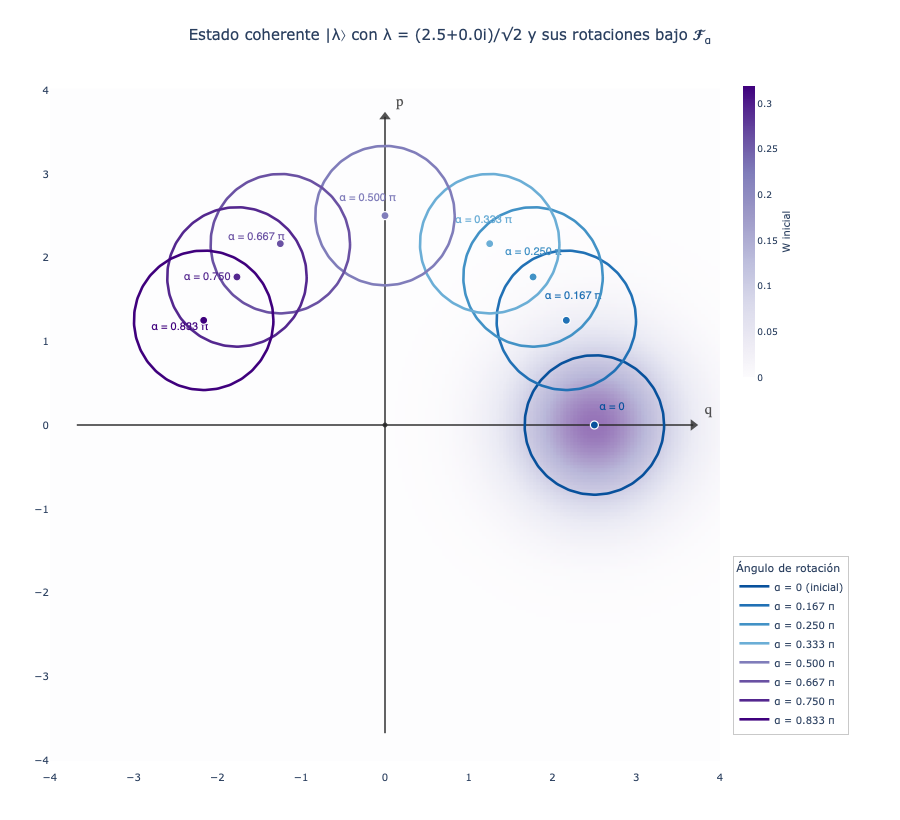
\includegraphics[width=0.6\textwidth]{Chapter3/Figures/TFFr_Coherents.png}
                    \caption{Distribución de Wigner de los estados coherentes rotados bajo la aplicación de la TFFr de distintos órdenes.}
                    \label{fig:TFFr-Coherentes}
                \end{figure}

                \subsubsection{Estados estrangulados del vacío}

                    Sea $\hat{S}(r) = \exp\left[r \left(\hat{a}^2 - \hat{a}^{\dagger 2}\right)/2 \right] $ con $r \in \mathbb{R}$ el operador de estrangulamiento \cite{stoler1970equivalence,Walls2008}, y sea $\ket{r} = \hat{S}(r)\ket{0}$ el vacío estrangulado (estrangulado a lo largo del eje $q$ con una varianza de $\hbar e^{-2r}/2$ en $\hat{q}$ y varianza de $\hbar e^{2r}/2$ en $\hat{p}$, tal que $\triangle q\triangle p = \hbar/2$ se preserva). La función de Wigner es una Gaussiana anisótropa 
                    \begin{equation}
                        W_{\ket{r}}\left(q,p\right) = \frac{1}{\pi\hbar} \exp\left[- \frac{e^{2r}q^2 + e^{-2r}p^2}{\hbar} \right].
                    \end{equation}

                    Aplicamos \ref{eq:Cap3TeoremaRotWigner} entonces
                    \begin{equation}
                        W_{\hat{\mathcal{F}}_\phi \ket{r}}(q,p) = \frac{1}{\pi\hbar}\exp\left[- \frac{1}{\hbar}\left( e^{2r}\left(q\cos\phi + p \sen\phi\right)^2 + e^{-2r}\left(-q\sen\phi + p \cos\phi \right)^2 \right) \right],
                    \end{equation}
                    expandiendo los cuadrados tenemos
                    \begin{equation*}
                        e^{2r} \left(q\cos\phi + p\sen\phi \right)^2 + e^{-2r} \left(q\sen\phi - p\cos\phi\right)^2  = Aq^2 + Bp^2 + 2C qp,
                    \end{equation*}
                    donde
                    \begin{align*}
                        & A = e^{2r}cos^2\phi + e^{-2r}\sen^2\phi, \\
                        & B = e^{2r}\sen^2\phi + e^{-2r}\cos^2\phi,\\
                        & C = \left(e^{2r} - e^{-2r}\right)\sen\phi \cos\phi = \sen h(2r)\sen\phi \cos\phi.
                    \end{align*}
                    Usando $\cos^2\phi = \left(1+\cos 2\phi\right)/2$ y $\sen^2\phi = \left(1- \cos 2\phi\right)/2$, los coeficientes se escriben como
                    \begin{align*}
                        & A = \cosh 2r + \sen h2r \cos 2\phi,\\
                        & B = \cosh 2r - \sen h2r \cos 2\phi,\\
                        & C = \sen h(2r)\sen\phi\cos\phi = \frac{1}{2}\sen h2r \sen 2\phi.
                    \end{align*}
                    Entonces la función de Wigner se escribe como
                    \begin{align}
                        & W_{\hat{\mathcal{F}}_\phi \ket{r}}(q,p) = \nonumber\\
                        &\frac{\pi}{\hbar} \exp\left\{-\frac{1}{\hbar} \left[ \left(\cosh 2r + \sen h 2r \cos 2\phi \right)q^2 + \left( \cosh 2r - \sen h2r \cos 2\phi \right)p^2 + \sen h2r \sen 2\phi\;qp \right]\right\}.
                    \end{align}

                    Entonces obtenemos que la elipse de los estados estrangulados originalmente alineada con el eje $q$ se rotó por un ángulo de $\phi$. Equivalentemente, podemos escribir
                    \begin{equation}
                        \hat{S}(r,\phi) = \hat{\mathcal{F}}_\phi \hat{S}(r) \hat{\mathcal{F}}_\phi^\dagger = \exp\left[ \frac{1}{2}r\left(\hat{a}^2e^{-2i\phi} - \hat{a}^{\dagger 2} e^{2i\phi} \right) \right],
                    \end{equation}
                    entonces la conjugación por $\hat{\mathcal{F}}_\phi$ produce la rotación rígida estándar del operador de estrangulamiento con parámetro $\zeta = re^{2u\phi}$ \cite{Walls2008,yuen1976two}. Esto muestra que la TFFr $\hat{\mathcal{F}}_\phi$ como el operador de orientación natural de la elipse de estrangulamiento en el espacio de fase como se muestra en la figura \ref{fig:TFFr-Squeezed}.

                    \begin{figure}[h]
                        \centering    
                        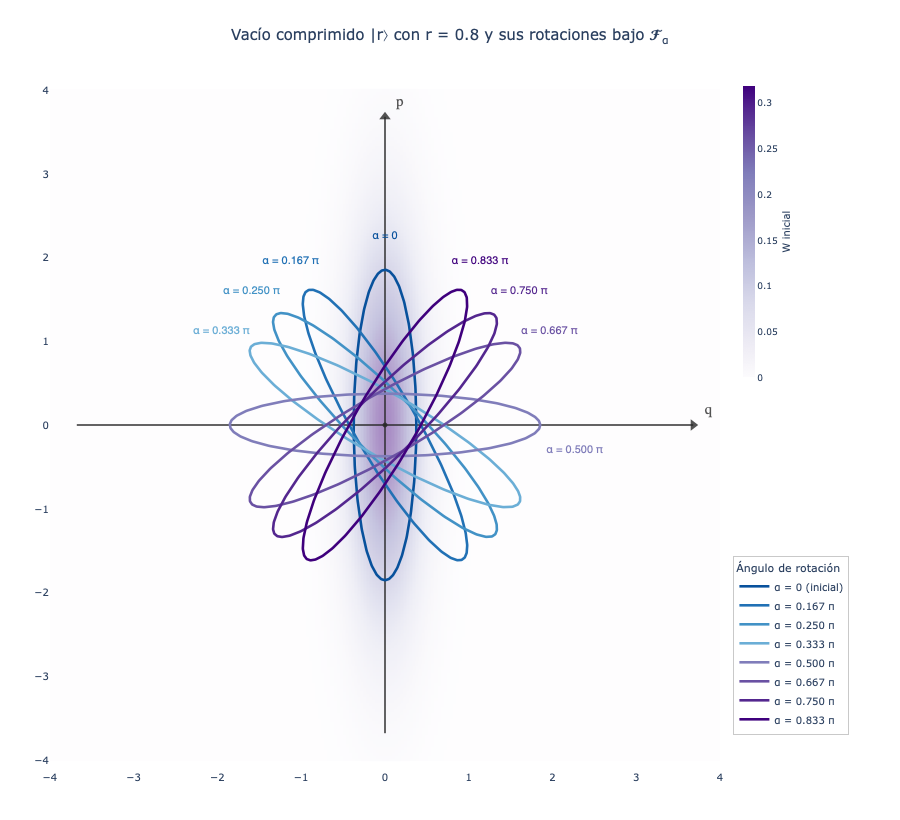
\includegraphics[width=0.6\textwidth]{Chapter3/Figures/TFFr_Squeezed.png}
                        \caption{Distribución de Wigner de los estados estrangulados del vacío rotados bajo la aplicación de la TFFr de distintos órdenes.}
                        \label{fig:TFFr-Squeezed}
                    \end{figure}
                \subsubsection{Estados de Fock}
                    
                    La función de Wigner para los estados número $\ket{n}$ es \cite{hillery1984distribution,cahill1969ordered,groenewold1946principles}
                    \begin{equation}
                        W_{\ket{n}}\left(q,p\right) = \frac{(-1)^n}{\pi\hbar} L_n\left(\frac{2\left(q^2 + p^2\right)}{\hbar} \right)e^{-\left(q^2+p^2\right)/\hbar},
                    \end{equation}
                    donde $L_n$ es el n-ésimo polinomio de Laguerre. Para $n=0$ se reduce a la función de Wigner del vacío, la cual coincide con una Gaussiana $W_{\ket{0}}(q,p) = (\pi\hbar)^{-1}\exp\left[-\left(q^2+p^2\right)/\hbar\right]$.

                    Vamos a aplicar entonces el teorema \ref{eq:Cap3TeoremaRotWigner}. Es importante notar que la función de Wigner de los estados de Fock $W_{\ket{n}}$ depende únicamente de la combinación radial $q^2+p^2$. Etonces, bajo la rotación tenemos
                    \begin{align*}
                        & q'^2 + p'^2 = \left(q\cos\phi + p\sen\phi \right)^2 + \left(-q\sen\phi + p\cos\phi \right)^2 \\
                        & = q^2\left(\cos^2\phi + \sen^2\phi \right) +2qp\left( \cos\phi\sen\phi - \sen\phi \cos\phi \right) = q^2 + p^2.
                    \end{align*}

                    Por lo tanto
                    \begin{equation}
                        W_{\hat{\mathcal{F}}_\phi \ket{n}} (q,p) = W_{\ket{n}}(q,p).
                    \end{equation}
                    Esto quiere decir que las funciones de Wigner de los estados de Fock son invariantes bajo la influencia de la Tranformación de Fourier Fraccionaria, lo cual, es completamente consisten con el operador desde su definición ya que
                    \begin{equation*}
                        \hat{\mathcal{F}}_\phi \ket{n} = e^{in\phi} \ket{n},
                    \end{equation*}
                    dado que el producto de un estado por una fase global deja a $\ket{n}\bra{n}$ (y por tanto a su función de Wigner) invariantes. Geométricamente (ver figura \ref{fig:TFFr-Fock}), los anillos concéntricos y las oscilaciones centrales de $W_{\ket{n}}$ poseen completa simetría respecto al origen.

                    \begin{figure}[h]
                        \centering    
                        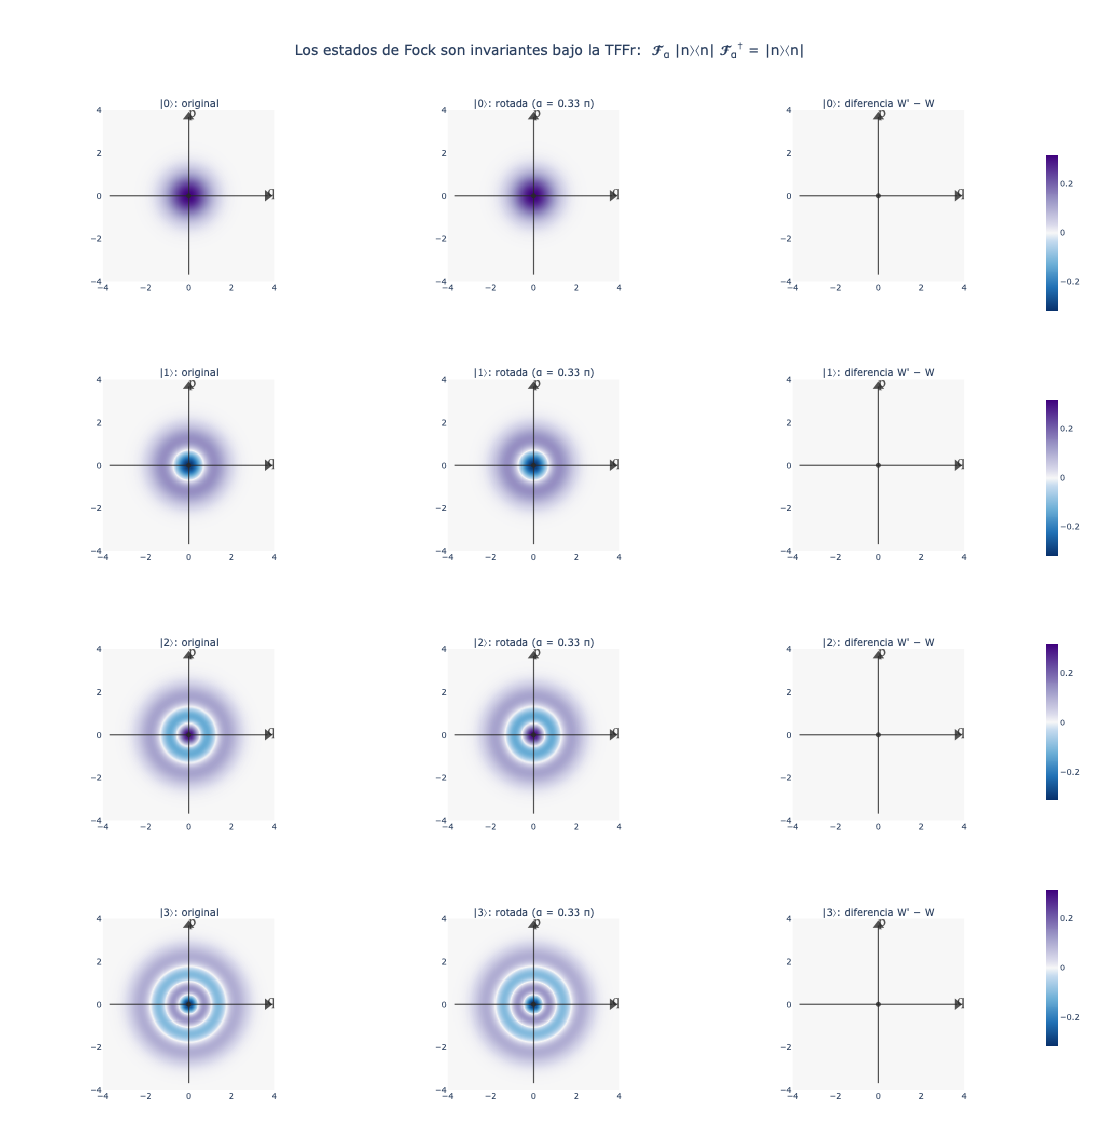
\includegraphics[width=0.6\textwidth]{Chapter3/Figures/TFFr_Fock.png}
                        \caption{Distribución de Wigner de los estados de Fock  bajo la aplicación de la TFFr de distintos órdenes, en donde podemos apreciar que se mantiene completamente invariante y tanto analítica como numéricamente su diferencia es cero.}
                        \label{fig:TFFr-Fock}
                    \end{figure}


                \subsubsection{Estados térmicos}

                    Un estado término para un valor medio de fotones de $\overline{n}$ es el estado mixto

                    \begin{equation}
                        \hat{\rho}_{th} = \frac{1}{\overline{n} + 1}\sum_{n=0}^{\infty} \left(\frac{\overline{n}}{\overline{n}+1}\right)^2 \ket{n}\bra{n},
                    \end{equation}
                    cuya función de Wigner \cite{hillery1984distribution,cahill1969density,Walls2008} es

                    \begin{equation}
                        W_{th}\left(q,p\right) = \frac{1}{\pi\hbar \left(2\overline{n} + 1\right)} \exp\left[- \frac{q^2+p^2}{\hbar\left(2\overline{n} + 1\right)}\right].
                    \end{equation}

                    Para $\overline{n} \to 0$, se reduce a la función de Wigner del vacío $W_{\ket{0}}$. Podemos ver que la variancia en cada cuadratura es de $\hbar\left(2\overline{n} + 1\right)/2$, la cual es $\hbar/2$ a temperatura cero y crece linealmente con $\overline{n}$.

                    Para aplicar el resultado \ref{eq:Cap3TeoremaRotWigner} observemso que la dependencia, nuevamente, es puramente radial: $q^2+p^2$. Por el mismo argument y resultado de los estados de Fock se tiene que $q'^2 + p'^2 = q^2 + p^2$, entonces

                    \begin{equation}
                        W_{\hat{\mathcal{F}}_\phi \hat{\rho}_{th}\hat{\mathcal{F}}_\phi^\dagger}(q,p) = W_{th}(q,p).
                    \end{equation}
                    Esto también es un poco esperable  ya que, a nivel de operadores, cada proyector $\ket{n}\bra{n}$ en la descomposición espectral de los estadso términos es invariantes bajo la TFFr $\hat{\mathcal{F}}_\phi$ (ver figura \ref{fig:TFFr-Termicos}y, por tanto, es una combinación convexa.
                    
                    \begin{figure}[h]
                        \centering    
                        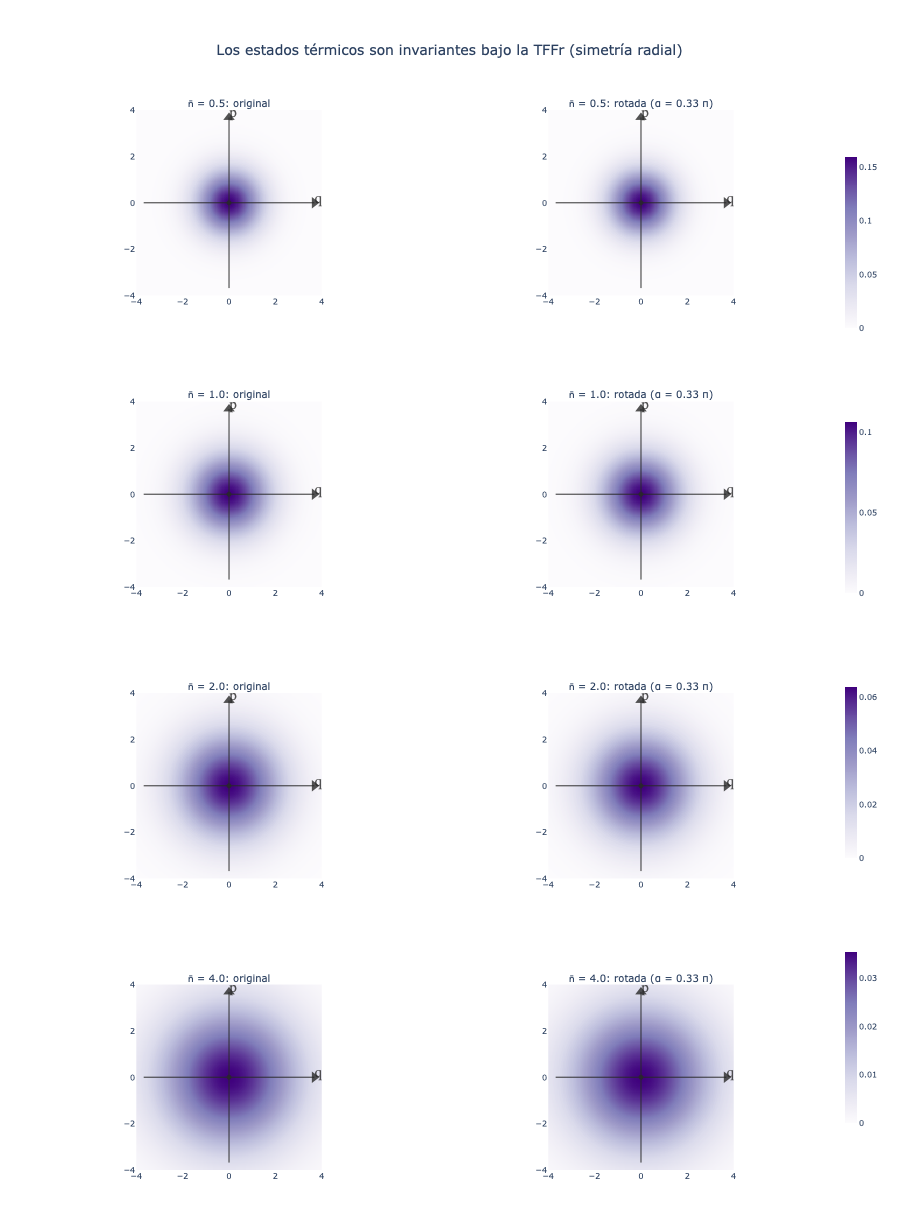
\includegraphics[width=0.6\textwidth]{Chapter3/Figures/TFFr_Termicos.png}
                        \caption{Distribución de Wigner de los estados de térmicos  bajo la aplicación de la TFFr de distintos órdenes, en donde podemos apreciar que se mantiene completamente invariante y, al igual que los estados de Fock, tanto analítica como numéricamente su diferencia es cero.}
                        \label{fig:TFFr-Termicos}
                    \end{figure}


    \section{Operador de fase cuántica}
                    
        Vamos a definir unos estados de fase escritos en la base de los estados número como
        \begin{equation*}\label{eq:Cap3EstadoNumeral}
            \ket{\#} = \sum_{n=0}^{\infty} \ket{n}.
        \end{equation*}

        Entonces, utilizando la $TFFr$ $\hat{\mathcal{F}}_\phi$ obtenemos
        \begin{equation}\label{eq:Cap3EStadosDeFase}
            \hat{\mathcal{F}}_\phi \ket{\#} = \sum_{n=0}^{\infty} e^{in\phi}\ket{n} = \ket{\phi}.
        \end{equation}

        Antes de seguir con el desarrollo matemático, veamos que geométricamente los estados $\ket{\#}$ representa un peine de Dirac la cual es la identidad de la suma de Poisson para el peine de Dirac de periodo $2\pi$ como se puede ver en la figura \ref{fig:Cap3-EstadoFase}, mientras que por el resultado \ref{eq:Cap3EStadosDeFase} el peine de Dirac (ver figura \ref{fig:Cap3-EstadoFaseRot}) se orienta dando origen a los estados de fase $\ket{\phi}$.

        \begin{figure}[htbp]
            \centering
            \begin{subfigure}[b]{0.45\textwidth}
                \centering
                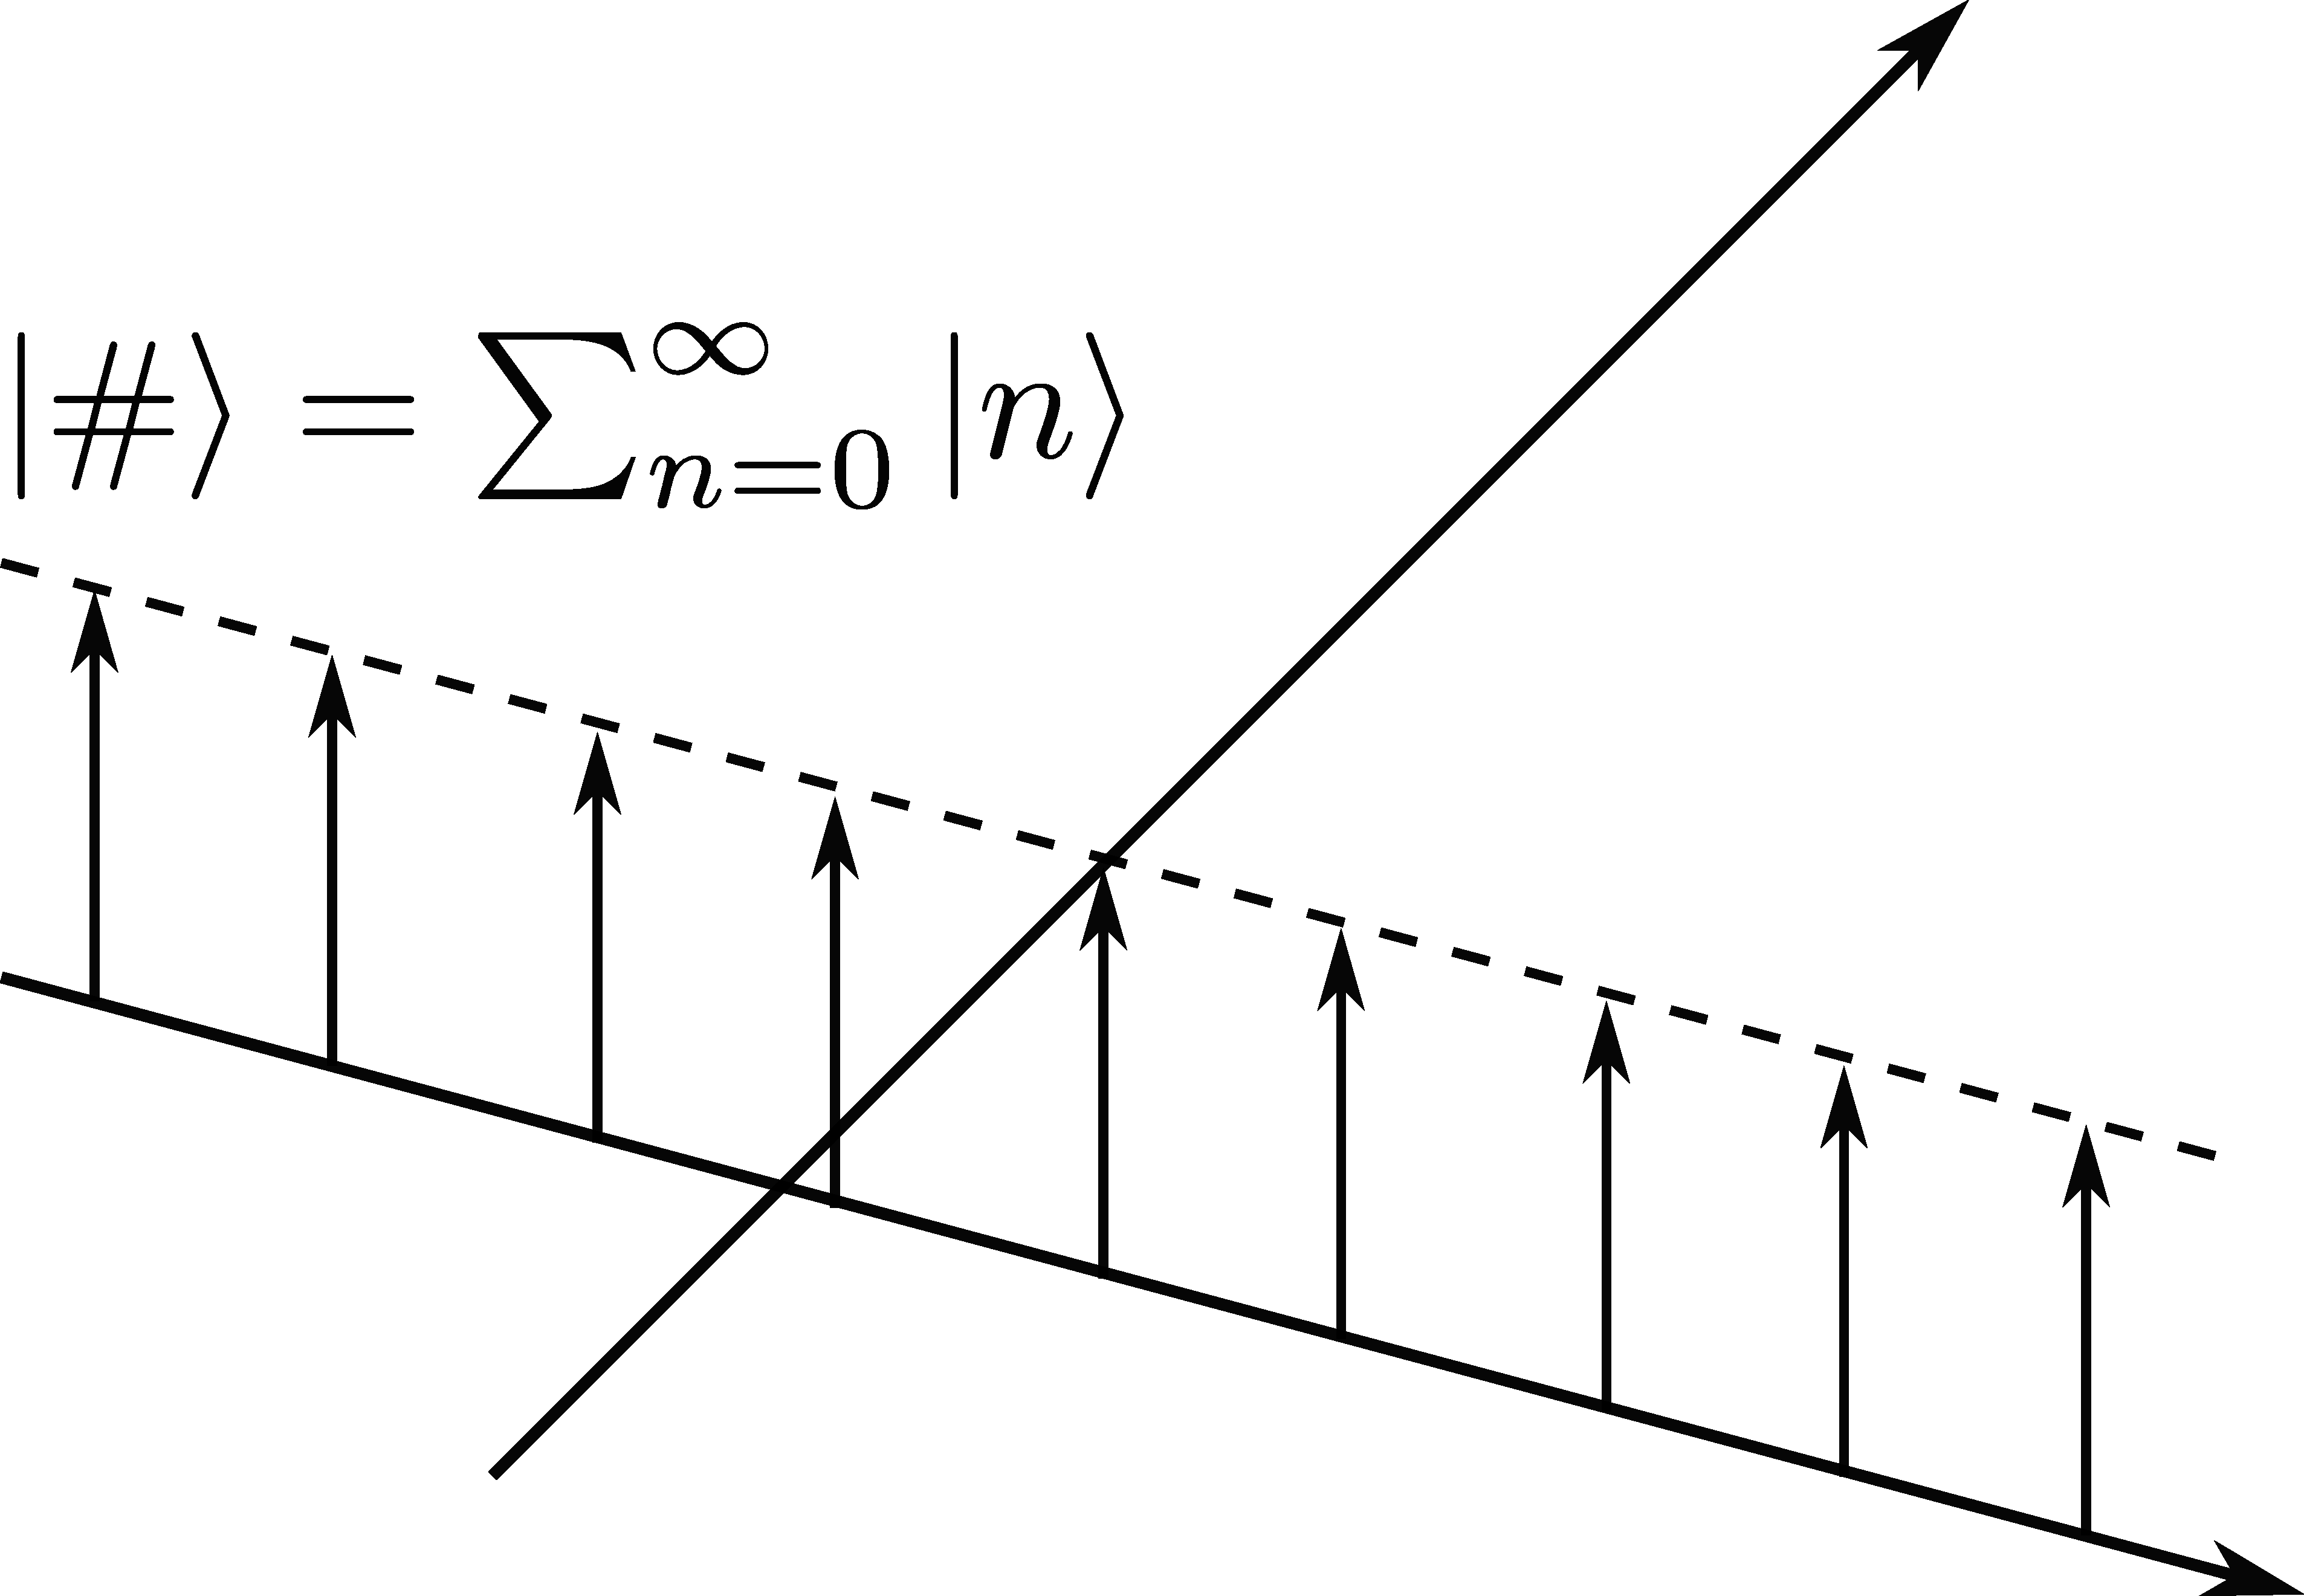
\includegraphics[width=\textwidth]{Chapter3/Figures/EstadosFase.pdf}
                \caption{Representación de los estados $\ket{\#}$ como peines de Dirac en el espacio de fase.}
                \label{fig:Cap3-EstadoFase}
            \end{subfigure}
            \hfill
            \begin{subfigure}[b]{0.45\textwidth}
                \centering
                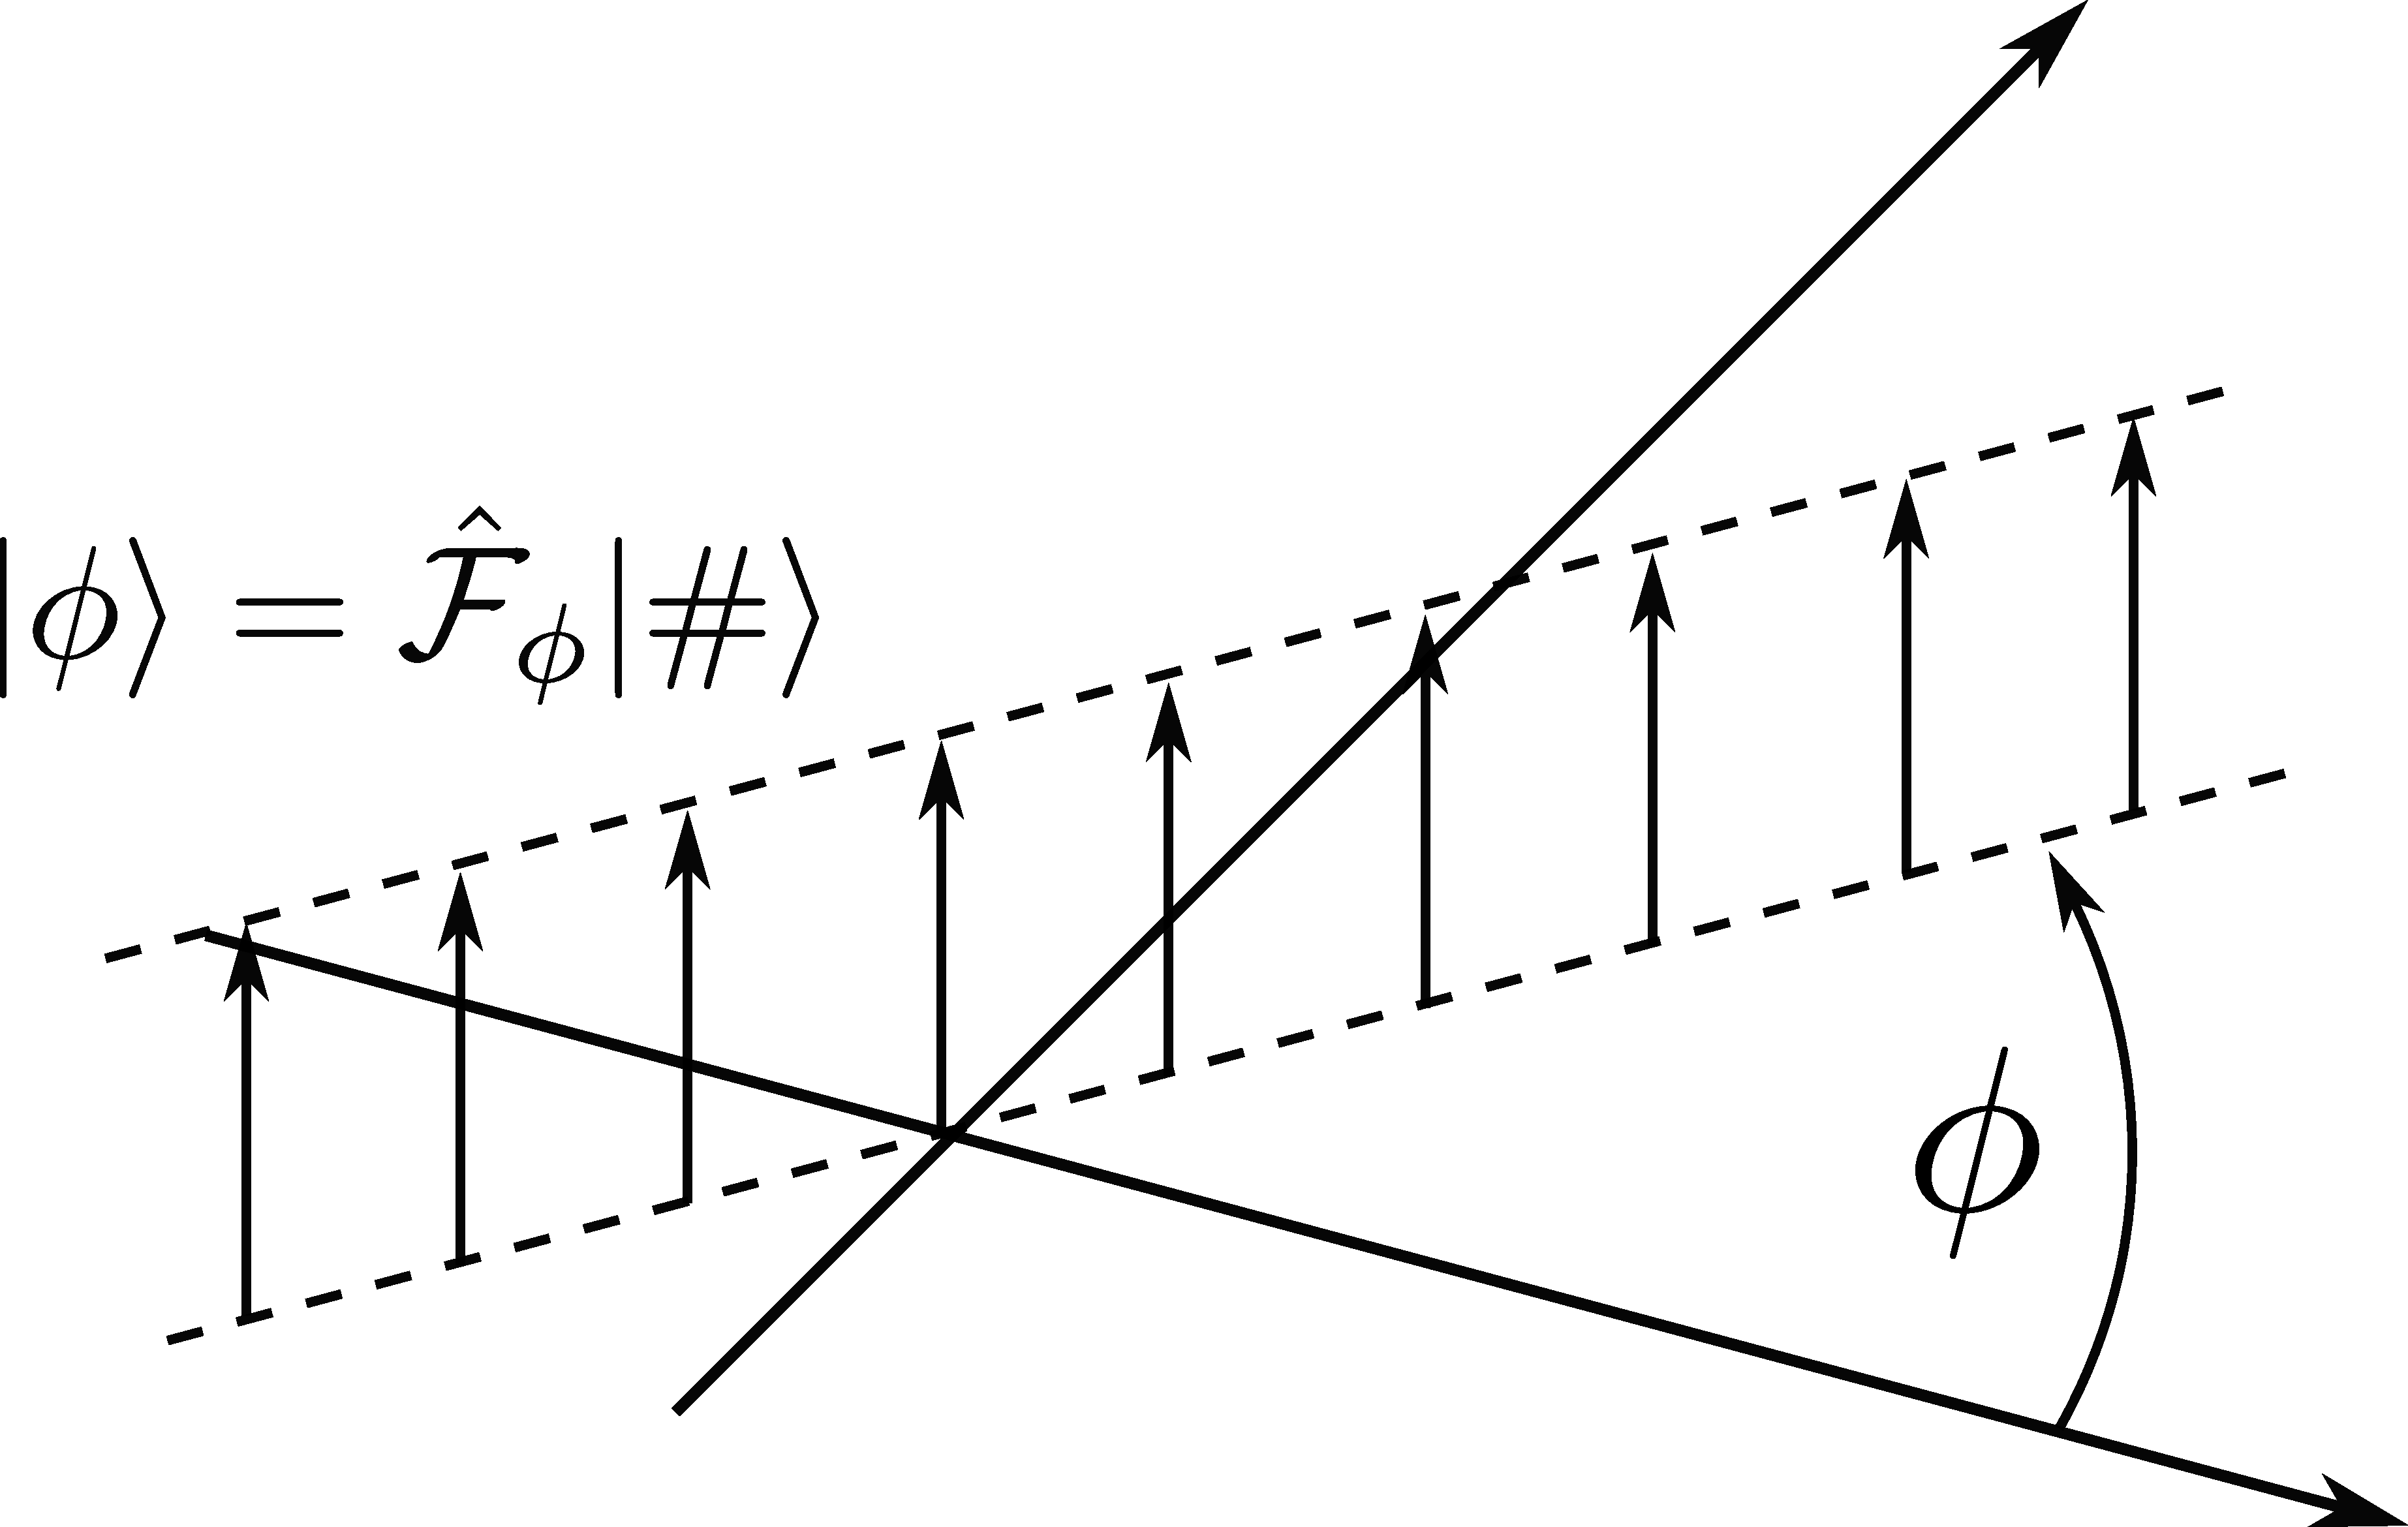
\includegraphics[width=\textwidth]{Chapter3/Figures/EstadosFase_Rot.pdf}
                \caption{Los estados de fase $\ket{\phi}$ corresponden a la aplicación de la TFFr de ordne $\phi$ sobre $\ket{\#}$ la cual, geométricamente, corresponde a orientar un ángulo $\phi$ el peine de Dirac.}
                \label{fig:Cap3-EstadoFaseRot}
            \end{subfigure}
            \caption{Represetanción de los estados de fase y su relación con la TFFr..}
            \label{fig:paralelo}
        \end{figure}

        Podemos ver que la no ortogonalidad de la familia de estados $\{\ket{\phi}\}$ es una manifestación del hecho de que cualesquiera dos estados de fase difieren por una rotación en el espacio de fase ($\hat{\mathcal{F}}_{\pm\theta}\ket{\phi} = \ket{\phi \pm \theta}$). 


        \subsection{Operadores Exponenciales de fase}

            De Sussking y Glogower \cite{susskind1964quantum}, introducimos los operadores exponenciales de fase de potencia $m$ escritos en la base de los estados número como
            \begin{equation}
                \hat{E}_m = \sum_{n=0}^{\infty}\ket{n}\bra{n+m}, \qquad m=0,1,2,3,...
            \end{equation}
            Donde $\hat{E}_0 = \hat{\mathcal{I}}$ y 
            \begin{equation}
                \hat{E}_m \ket{\phi} = e^{im\phi}\ket{\phi}.
            \end{equation}
            De hecho,
            \begin{equation*}
                \hat{E}_m \ket{\phi} = \sum_{n,k=0}^{\infty} \ket{n}\bra{n+m}e^{ik\phi}\ket{k} = \sum_{_n=0}^{\infty}e^{i(n+m)\phi}\ket{n} = e^{im\phi}\ket{\phi},
            \end{equation*}
            y sobre los estadso número opera como
            \begin{equation}
                \hat{E}_m \ket{n} = 
                \left\{
                \begin{matrix}
                    \ket{n-m}, & n \geq m\\
                    0, & n < m
                \end{matrix}
                \right.
                \qquad \hat{E}_m^\dagger \ket{n} = \ket{n+m}.
            \end{equation}
            Un cambio en los índices mudos nos da
            \begin{equation*}
                \sum_{n=m}^{\infty} \ket{n}\bra{n-m} = \sum_{n=0}^{\infty}\ket{n+m}\bra{n} = \hat{E}^\dagger_m.
            \end{equation*}

            Estos operadores exponenciales de fase heredan la semi-unitareidad de la formulación original de Sussking-Glogower, en donde se tiene que
            \begin{align}
                & \hat{E}_m \hat{E}_m^\dagger = \sum_{n,n'=0}^{\infty} \ket{n}\braket{n+m|n'+m} \bra{n'} = \hat{\mathcal{I}},\\
                & \hat{E}_m^\dagger\hat{E}_m = \sum_{n=0}^{\infty} \ket{n+m}\bra{n+m} = \hat{\mathcal{I}}- \sum_{n=0}^{m-1}\ket{n}\bra{n}.
            \end{align}

            Entonces el conmutador de los exponenciales de fase es
            \begin{equation*}
                \left[\hat{E}_m, \hat{E}_m^\dagger\right] = \sum_{n=0}^{m-1}\ket{n}\bra{n}.
            \end{equation*}

            Veamos ahora cómo relacionar la TFFr con estos operadores exponenciales y sus reglas de conmutación.  Dado que, en la base de los estados número $\hat{\mathcal{F}}_\theta = \sum_{n=0}^{\infty} e^{in\theta}\ket{n}\bra{n}$ es diagonal, entonces
            \begin{align*}
                & \hat{E}_m \hat{\mathcal{F}}_\theta = \sum_{n=0}^{\infty} e^{i(n+m)\theta}\ket{n}\bra{n+m},\\
                & \hat{\mathcal{F}}_\theta \hat{E}_m = \sum_{n=0}^{\infty} e^{in\theta}\ket{n}\bra{n+m},
            \end{align*}
            luego los conmutadores son entonces
            \begin{align}
                & \left[\hat{E}_m, \hat{\mathcal{F}}_\theta\right] = \left(e^{im\theta} - 1\right)\hat{\mathcal{F}}_\theta \hat{E}_m, \\
                & \left[\hat{E}_m^\dagger, \hat{\mathcal{F}}_\theta\right] = \left(1-e^{im\theta}\right)\hat{E}_m^\dagger \hat{\mathcal{F}}_\theta.
            \end{align}

            Vamos a usar estos conmutadores para calcular las transformaciones de similaridad de los exponenciales de fase. Del primer conmutador tenemos que $\hat{E}_m\hat{\mathcal{F}}_\theta = e^{im\theta} \hat{\mathcal{F}}_\theta \hat{E}_m$, tendremos
            \begin{equation}\label{eq:Cap3SimilaridadEm}
                \hat{\mathcal{F}}_\theta \hat{E}_m \hat{\mathcal{F}}_\theta^\dagger = e^{-im\theta} \hat{E}_m, \qquad \hat{\mathcal{F}}_\theta \hat{E}_m^\dagger \hat{\mathcal{F}}_\theta^\dagger = e^{im\theta} \hat{E}_m^\dagger,
            \end{equation}
            y al actuar sobre un estado de fase $\ket{\phi}$ tendremos que la TFFr rota los estados de fase en un ángulo $\theta$
            \begin{equation}
                \hat{\mathcal{F}}_\theta \hat{E}_m \hat{\mathcal{F}}_\theta^\dagger \ket{\phi} = e^{im(\phi-\theta)}\ket{\phi}.
            \end{equation}
        
        \subsection{Operador hermítico de fase}
            
            Toda la construcción previa se susstenta en la construcción de las herramientas suficientes para usar al construcción de Toeplitz-Rosenblum y así obtener un operador de fase hermítico. Primero, vamos a calcular el projecto de fase cero $\ket{\#}\bra{\#}$ el cual, en la base de los estados número, acepta la descomposición
            \begin{equation}
                \ket{\#}\bra{\#} = \sum_{n,n'=0}^{\infty} \ket{n}\bra{n'} = \sum_{m=-\infty}^{^\infty} \hat{E}_m = \sum_{n=0}^{\infty}\ket{n}\bra{n} + \sum_{m=1}^{\infty} \left(\hat{E}_m + \hat{E}_m^\dagger\right).
            \end{equation}
            Donde hemos utilizado que $\hat{E}^{-m} = \hat{E}_m^\dagger$ y $\hat{E}_0 = \hat{\mathcal{I}}$. Conjugación con la TFFr $\hat{\mathcal{F}}_\theta$ y utilizando \ref{eq:Cap3SimilaridadEm}
            \begin{equation}\label{eq:Cap3ProyectorTheta}
                \ket{\theta}\bra{\theta} = \hat{\mathcal{I}} + \sum_{m=1}^{\infty} \left(e^{-im\theta}\hat{E}_m + e^{im\theta} \hat{E}_m^\dagger \right).
            \end{equation}

            Dado que la familia $\{\ket{\phi}\}$ no son ortogonales, adoptaremos al construcción de Toeplitz-Rosenblum \cite{rosenblum1962self}. Dado $f \in \mathbb{L}^1(\mathbb{R})$ se tiene que un operador Hermítico $\hat{F}_\phi$ está dado por
            \begin{equation}
                \hat{F}_\phi = \frac{1}{2\pi} \int_{\phi}^{\phi+2\pi} f(\theta)\ket{\theta}\bra{\theta}d\theta.
            \end{equation}

            Escogiendo $f(\theta) = \theta$ obtenemos un operador tipo Garrison-Wong \cite{Garrison1970}. Sustituyendo \ref{eq:Cap3ProyectorTheta}, tendremos las siguientes tres integrales

            \begin{equation}
                I_0 = \frac{1}{2\pi}\int_\phi^{\phi+2\pi} \theta d\theta, \qquad I_\pm  = \frac{1}{2\pi}\int_\phi^{\phi+2\pi}\theta e^{\pm im\theta}d\theta.
            \end{equation}

            La primera integral es inmdiata
            \begin{equation*}
                I_0 = \frac{(\phi+2\pi)^2 - \phi^2}{4\pi} = \phi+\pi.
            \end{equation*}
            Para las otras dos integrales, mediante integrcación por partes $(u=\theta, dv=e^{\pm im\theta}d\theta)$nos da, después de usar $e^{\pm im(\phi+2\pi)} = e^{\pm im\phi} (m\in \mathbb{Z})$
            \begin{equation*}
                I_\pm  = \frac{1}{2\pi} \left[\frac{\theta e^{\pm im\theta}}{\pm im}|_\phi^{\phi+2\pi} - \frac{1}{\pm im}\int_\phi^{\phi +2\pi} e^{\pm im\theta}d\theta  \right] = \frac{1}{2\pi} \frac{2\pi e^{\pm im\theta}}{\pm im} - 0 = \mp \frac{ie^{\pm im\phi}}{m}.
            \end{equation*}
            Entonces tenemos que el operador de fase $\hat{\Theta_\phi}$ es
            \begin{equation}\label{eq:Cap3OperadorFaseHermitico}
                \hat{\Theta}_\phi = (\phi + \pi)\sum_{n=0}\ket{n}\bra{n} + i \sum_{n=1}^\infty \frac{e^{-im\phi}}{m}\hat{E}_m -i\sum_{m=1}^{\infty} \frac{e^{im\phi}}{m}\hat{E}_m^\dagger.
            \end{equation}
            Usando $\hat{\mathcal{F}}_\phi \ket{n}\bra{n+m}\hat{\mathcal{F}}_\phi^\dagger = e^{-im\phi}\ket{n}\bra{n+m}$ y la relación análoga para el conjugado, entonces el operador de fase adquiere la forma
            \begin{equation}\label{eq:Cap3OperadorFaseHermiticoFourier}
                \hat{\Theta}_\phi = (\phi+\pi)\hat{\mathcal{I}} + i \hat{\mathcal{F}}_\phi \left(\sum_{m=1}^{\infty}\sum_{n=0}^{\infty}\frac{\ket{n}\bra{n+m} - \ket{n+m}\bra{n}}{m} \right)\hat{\mathcal{F}}_\phi^\dagger.
            \end{equation}

            Si hacemos $\phi = -\pi$ en la ecuación \ref{eq:Cap3OperadorFaseHermitico} y usando $e^{\mp im\pi}=(-1)^m$, tendremos
            \begin{equation}\label{eq:Cap3OperadorFaseMenosPi}
                \hat{\Theta}_{-\pi} = i \sum_{m=1}^{\infty}\sum_{n=0}^{\infty} \frac{(-1)^m}{m}\left(\ket{n}\bra{n+m} - \ket{n+m}\bra{n} \right),
            \end{equation}
            y podemos ver así que, el operador de fase, consiste en tomar el proyector de estados de fase $-\pi$ y rotarlos un ángulo de $\phi$ mediante una transformación de similaridad de la TFFr y así, dado una referencia $\phi$ el operador $\hat{\Theta}_\phi$ es hermítico lo cual coincide con el formalismo de Wong \cite{Garrison1970} y la formulación de operadores de fase de \cite{Bergou1991} \textbf{ACÁ DEBO VOLVER A REVISAR CON CALMA EL PAPER Y VER QUÉ TIENEN DE SEMEJANTES}.

            Dado que la base de estados de fase no son ortogonales, el cuadrado de operadores de fase no es el cuadrado del operador de fase, es decir $\hat{\Theta}_\phi^2 \neq \left(\hat{\Theta}_\phi\right)^2$ en general; el operador cuadrático debe ser definido mediante la contrucción de Toeplitz-Rosenblum con $f(\theta) = \theta^2$. Necesitamos calcular

            \begin{equation*}
                J_0 = \frac{1}{2\pi}\int_\phi^{\phi+2\pi} \theta^2 d\theta, \qquad J_\pm = \frac{1}{2\pi} \int_\phi^{\phi+2\pi} \theta^2e
                {\pm im\theta}d\theta.
            \end{equation*}

            Calculando directamente obtenemos
            \begin{equation*}
                J_0 = \frac{\left(\phi + 2\pi\right)^3 - \phi^3}{6\pi} = (\phi + \pi)^2 + \frac{\pi^2}{3}, \qquad J_\pm = 2\left[\mp \frac{i(\phi + \pi)}{m} + \frac{1}{m^2} \right]e^{\pm im\phi}, 
            \end{equation*}
            y así el operador cuadrático de fase es
            \begin{align}\label{eq:Cap3OperadorHermiticoFaseCuadradoFourier}
                & \hat{\Theta}_\phi^2 = \left[(\phi + \pi)^2 + \frac{\pi^2}{3} \right]\hat{\mathcal{I}} + 2(\phi + \pi)\hat{\mathcal{F}}_\phi \sum_{m=1}^{\infty}\sum_{n=0}^{\infty}\frac{\ket{n}\bra{n+m} - \ket{n+m}\bra{n}}{m} \hat{\mathcal{F}}_\phi^\dagger \nonumber\\
                & + 2\hat{\mathcal{F}}_\phi \sum_{m=1}^{\infty}\sum_{n=0}^{\infty}\frac{\ket{n}\bra{n+m} + \ket{n+m}\bra{n}}{m^2} \hat{\mathcal{F}}_\phi^\dagger,
            \end{align}
            en donde podemos ver que si $\phi = -\pi$ tenemos
            \begin{equation}
                \hat{\Theta}_{-\pi}^2 = \frac{\pi^2}{3}\hat{\mathcal{I}} + 2 \sum_{m,n}^{\infty}\frac{(-1)^m}{m^2}\left(\ket{n}\bra{n+m} + \ket{n+m}\bra{n} \right),
            \end{equation}
            y así, el operador de fase al cuadrado consiste en una fase escalar, una rotación de $\phi$ del operador $\hat{\Theta}_{-\pi}$ y otra rotación de $\phi$ del operador cuadrático $\hat{\Theta}_{-\pi}^2$. 

            Hasta este momento, todo lo desarrollado ha sido para construir un operador de fase hermítico en espacios de Hilbert de dimensión infinita sin la necesidad de introducir un espectro negativo tal como lo hacen Pegg y Barnett, sin embargo, este desarrollo reproduce los resultados de \cite{Bergou1991} en su totalidad, por lo tanto, lo que se muestra en este trabajo es una reformulación de estos operadores en donde utilizando la TFFr queda más claro la perspectiva geométrica y naturaleza tanto de los estados de fase como la construcción de los operadores de fase y replicaremos el conmutador de London que, como ya se mostró, es matemáticamente inconsistente tener un conmutador canónico entre el operador número y el operador de faes. Calculemos entonces este conmutador en donde, por brevedad y sin pérdida de generalidad diremos $\hat{\Theta} \equiv \hat{\theta}_{-\pi}$ entonces

            \begin{align*}
                & \hat{N}\hat{\Theta} = \sum_{k=0}^{\infty} k \ket{k}\bra{k} \cdot i \sum_{m,n}^{\infty} \frac{(-1)^m}{m}\left(\ket{n}\bra{n+m} - \ket{n+m}\bra{n}\right)\\
                & = i\sum_{m,n}^{\infty}\frac{(-1)^m}{m}\left[n\ket{n}\bra{n+m} - (n+m)\ket{n+m}\bra{n} \right], \\
                & \hat{\Theta}\hat{N} = i \sum_{m,n}^{\infty} \frac{(-1)^m}{m}\left(\ket{n}\bra{n+m} - \ket{n+m}\bra{n}\right)\sum_{k}^{\infty} k \ket{k}\bra{k}\\
                & = i \sum_{m,n}^{\infty} \frac{(-1)^m}{m}\left[(n+m)\ket{n}\bra{n+m} - n\ket{n+m}\bra{n} \right],
            \end{align*}
            restando tendremos que el conmutador es
            \begin{equation}
                \left[\hat{N}, \hat{\Theta}\right] = -i \sum_{m=1}^{\infty}\sum_{m=0}^{\infty} (-1)^m \left(\ket{n}\bra{n+m} + \ket{n+m}\bra{n} \right).
            \end{equation}

            Del proyector de fase \ref{eq:Cap3ProyectorTheta} para $\theta = \pi$ y usando $e^{\pm im\pi} = (-1)^m$ 
            \begin{align*}
                & \ket{\pi}\bra{\pi} = \hat{\mathcal{I}} + \sum_{m=1}^{\infty} (-1)^m \left(\hat{E}_m + \hat{E}_k^\dagger \right),\\
                & \hat{\mathcal{I}} - \ket{\pi}\bra{\pi} = - \sum_{m,n}^{\infty} (-1)^m \left(\ket{n}\bra{n+m} + \ket{n+m}\bra{n} \right),
            \end{align*}
            ell cual coincide con el lado derecho de la ecuación que representa al conmutador divido por $i$, entonces
            \begin{equation}\label{eq:Cap3ConmutadorNTheta}
                \left[\hat{N}, \hat{\Theta}\right] = i \left(\hat{\mathcal{I}} - \ket{\pi}\bra{\pi} \right).
            \end{equation}

            El conmutador \ref{eq:Cap3ConmutadorNTheta} es la forma de Judge-Lewis \cite{judge1963commutator}, donde $\hat{Theta}$ es un operador de ángulo de periodo $2\pi$. Acá se obtiene sin hacer ninguan extensión del espacio de Hilbert a estados número negativos. El estado $\ket{\pi}$ es no normalizable; el projector $\ket{\pi}\bra{\pi}$ en realidad se porta como una distribución delta de Dirac de periodo $2\pi$ es decir $\delta_{2\pi}(\theta-\pi)$ en la representación de fase.

        \subsection{Operadores de fase para distintos estados cuánticos}
            
            En esta sección vamos a calcular los valores esperados $\braket{\hat{\Theta}}$ y $\braket{\hat{\Theta}^2}$ para distintos estados y dar su interpretación física y matemática.

            \subsubsection{Estados de Fock}

                Para los estados número $\ket{n}$\ref el valor esperado de la ecuación \ref{eq:Cap3OperadorFaseHermiticoFourier} nos da
                \begin{equation}
                    \bra{n}\hat{\Theta}_\phi \ket{n} = \left(\phi + \pi\right) + i \bra{n} \hat{\mathcal{F}}_\phi \left( \sum_{m=1}^{\infty}\sum_{n=0}^{\infty}\frac{\ket{n}\bra{n+m} - \ket{n+m}\bra{n}}{m}  \right)\hat{\mathcal{F}}_\phi^\dagger \ket{n},
                \end{equation}
                dado que $\hat{\mathcal{F}}_\phi \ket{n} = e^{-in\phi}\ket{n}$ y el término que está bajo la transformación de similaridad está fuersa de la diagonal en la base de Fock, entonces $\bra{n} \hat{\mathcal{F}}_\phi \left( \sum_{m=1}^{\infty}\sum_{n=0}^{\infty}\frac{\ket{n}\bra{n+m} - \ket{n+m}\bra{n}}{m}  \right)\hat{\mathcal{F}}_\phi^\dagger \ket{n} = 0$ y el valor esperado del operador de fase es
                \begin{equation}
                    \bra{n} \hat{\Theta}_\phi \ket{n} = \phi + \pi.
                \end{equation}

                Análogamente, de \ref{eq:Cap3OperadorHermiticoFaseCuadradoFourier} tenemos
                \begin{equation}
                    \bra{n}\hat{\phi}^2_\phi \ket{n} = \left(\phi + \pi\right)^2 + \frac{\pi^2}{3}.
                \end{equation}
                Por lo tanto, la varianza será
                \begin{equation}
                    \triangle \hat{\Theta}_\phi^2 = \bra{n}\hat{\Theta}_\phi^2\ket{n} - \bra{n}\hat{\Theta}_\phi\ket{n}^2 = \frac{\pi^2}{3},
                \end{equation}
                la cual corresponde correctamente a la varianza de una distribución de fase uniforme en un intervalo de longitud $2\pi$, $\sigma^2 = (2\pi)^2/12 = \pi^2/3$, consistente con el hecho de que los estados de Fock tienen una fase indeterminada.

            \subsubsection{Estados de Fase}
                
                Ahora vamos a evaluar $\hat{\Theta} \equiv \hat{\Theta}_{-\pi}$ sobre los estados de fase $\ket{\phi}$ y vamos a demostrar que recuperaremos la identidad $\hat{\Theta}\ket{\phi} = \phi \ket{\phi}\; $ para cada $\pi \in \left(-\pi,\pi\right)$. De \ref{eq:Cap3OperadorFaseMenosPi} tenemos
                \begin{align*}
                    & \hat{\Theta}\ket{n} = i \sum_{m=1}^{n}\frac{(-1)^m}{m}\ket{n-m} - i \sum_{m=1}^{\infty} \frac{(-1)^m}{m}\ket{n+m} = i \sum_{k\neq n}^{\infty} \frac{(-1)^{n-k}}{n+k}\ket{k},
                \end{align*}
                en donde, en el último paso, se hizo el cambio de variables $k= n-m$ en la primera suma y $k= n+m$ en la segunda. En particular
                \begin{equation*}
                    \bra{n}\hat{\Theta}\ket{n} = 0,
                \end{equation*}
                el cual es el caso especial cuando $\phi = -\pi$ de la varianza del operador de fase en la base de Fock ya que $\phi + \pi = 0$.

                Vamos a calcular los elementos de matriz
                \begin{align*}
                    \bra{m}\hat{\Theta}\ket{\phi} = \sum_{n=0}^{\infty} e^{in\phi} \bra{m}\hat{\Theta}\ket{n} = i \sum_{n\neq m}^{\infty} \frac{(-1)^{n-m}}{n+m}e^{in\phi} = ie^{im\phi} \sum_{l=-m, l \neq 0}^{\infty} \frac{(-1)^l}{l}e^{il\phi},
                \end{align*}
                donde $l=n-m$.  Para dar uan cara explícita, veamos que la serie de Fourier para la función diente de sierra de periodo $2\pi$ $f(\phi) = \phi$ en $(-\pi,\pi)$ es
                \begin{equation*}
                    \phi = i \sum_{l\neq 0, l \in \mathbb{Z}}^{\infty} \frac{(-1)^l}{l}e^{il\phi}, \quad -\pi < \phi < \phi.
                \end{equation*}

                Entonces, en el límite formal donde la cota inferior $-m$ en  la serie de Fourier de la sierra puede ser reemplazada por $-\infty$ (el cua lse justifica en los elementos de matriz con suficientes estados suaves),
                \begin{equation}
                    \bra{m}\hat{\Theta}\ket{\phi} \longrightarrow \phi e^{im\phi} = \phi \braket{m|\phi},
                \end{equation}
                por lo tanto
                \begin{equation}
                    \hat{\Theta}\ket{\phi} = \phi \ket{\phi}, \quad -\pi < \phi < \pi.
                \end{equation}

            \subsubsection{Estados coherentes}
                
                Sea $\ket{\lambda}$ con $\lambda = |\lambda|e^{i\theta}$. De \ref{eq:Cap3OperadorFaseHermiticoFourier}
                \begin{align}
                    & \bra{\lambda} \hat{\Theta}_\phi \ket{\lambda} = (\phi + \pi) + i \bra{\lambda}\hat{\mathcal{F}_\phi} \left( \sum_{m=1}^{\infty}\sum_{m=0}^{\infty} \frac{\ket{n}\bra{n+m} - \ket{n+m}\bra{n}}{m} \right) \hat{\mathcal{F}}_\phi^\dagger  \ket{\lambda} \nonumber\\
                    & = (\phi + \pi) + i \bra{\mu} \frac{\ket{n}\bra{n+m} - \ket{n+m}\bra{n}}{m} \ket{\mu},
                \end{align}
                donde $\mu = \lambda e^{-i\phi} = |\lambda| e^{i(\theta-\phi)}$. Para un estado coherente $\mu$ tenemos
                \begin{equation*}
                    \braket{\nu | n} = e^{- \frac{|\mu|^2}{2}}\frac{(\mu^*)^n}{\sqrt{n!}},
                \end{equation*}
                entonces
                \begin{align*}
                    & \bra{\mu} \left(\ket{n}\bra{n+m}\right)\ket{\mu} = e^{-|\mu|^2} \frac{(\mu^*)^n \mu^{n+m}}{\sqrt{n!(n+m)!}} = e^{-|\lambda|^2} \frac{|\lambda|^{2n+m}e^{im(\theta-\phi)}}{\sqrt{n!(n+m)!}},
                \end{align*}
                y el término transpuesto nos da el complejo conjugado, por tanto que en la base de los estados coherentes $\ket{\mu}$
                \begin{align}
                    & \bra{\mu}\sum_{m=1}^{\infty}\sum_{m=0}^{\infty} \frac{\ket{n}\bra{n+m} - \ket{n+m}\bra{n}}{m} \ket{\mu} = e^{-|\lambda|^2} \sum_{m=1}^{\infty} \frac{2i \sen\left[m\left(\theta-\phi\right)\right]}{m}S_m\left(|\lambda|\right) \nonumber\\
                    & S_m(r) = \sum_{n=0}^{\infty} \frac{r^{2n+m}}{\sqrt{n!(n+m)!}},
                \end{align}
                juntando todo, el valor esperado del operadro de fase en la base de los estados coherentes es
                \begin{equation}
                    \bra{\lambda}\hat{\Theta}_\phi \ket{\lambda} = (\phi + \pi) - 2e^{-|\lambda|^2} \sum_{m=1}^{\infty} \frac{\sen\left[m(\theta-\phi)\right]}{m}S_m\left(|\lambda|\right).
                \end{equation}

                La idea central es probar que en el límite clásico, cuando $|\lambda| \to \infty$ se recupera la fase clásica. En este límite, las funciones $S_m(|\lambda|)$ tienen una forma cerrada conocida relacionada con las funciones de Bessell \cite{cahill1969ordered}
                \begin{equation*}
                    S_m(r) = I_m(2r^2),
                \end{equation*}
                o de manera más precisa, definiendo $\tilde{S}_m(r) = e^{-r^2}S_m(r)$ y usando la identidad de la función generatriz

               \begin{equation}
                    \sum_{n=0}^{\infty} \frac{r^{2n+m}}{\sqrt{n!(n+m)!}} \overset{r\to \infty}{\longrightarrow} e^{r^2} \left(1 - \frac{m^2}{4r^2} + \mathcal{O}(r^{-4})\right),
               \end{equation}
               se obtiene que $e^{-|\lambda|^2}S_m(|\lambda|) \to 1$ cuando $|\lambda| \to \infty$. En este límite, el valor esperado se reduce a
               \begin{equation}
                    \bra{\lambda} \hat{\Theta}_\phi \ket{\lambda} \overset{|\lambda|\to \infty}{\longrightarrow} (\phi + \pi) - 2\sum_{m=1}^{\infty} \frac{\sen\left(m(\theta-\phi)\right)}{m},
               \end{equation} 
               la cual corresponde a la serie de Fourier de la función diente de sierra de periodo $2\pi$. Concretamente, usando la identidad
               \begin{equation}
                   2\sum_{m=1}^{\infty}\frac{\sen(m\xi)}{m} = \pi - \xi, \quad 0 < \xi < 2\pi,
               \end{equation}
               con $\xi = \theta - \phi \in (0,2\pi)$, obtenemos directamente
               \begin{equation}
                   \bra{\lambda}\hat{\Theta}_\phi\ket{\lambda} \overset{|\lambda|\to\infty}{\longrightarrow} (\phi+\pi) - \left(\pi - (\theta-\phi)\right) = \theta,
               \end{equation}
               de modo que, en el límite clásico, el operador de fase recupera exactamente la fase clásica $\theta = \arg\lambda$ del estado coherente, con independencia de la referencia $\phi$.

               Para la varianza, un cálculo análogo a partir del operador cuadrático \ref{eq:Cap3OperadorHermiticoFaseCuadradoFourier} con $\phi = -\pi$ conduce, para $|\lambda|\gg 1$, a
               \begin{equation}\label{eq:Cap3VarianzaCoherentes}
                   \Delta\hat{\Theta}^2 \approx \frac{1}{4|\lambda|^2} = \frac{1}{4\bar{n}},
               \end{equation}
               donde $\bar{n} = |\lambda|^2$ es el número medio de fotones. Este resultado reproduce la incertidumbre de fase semiclásica estándar y es completamente consistente con el producto de incertidumbre número-fase $\Delta N\cdot\Delta\hat{\Theta}\approx\frac{1}{2}$ para estados mínimos en el régimen de muchos fotones \cite{Barnett1989,Lynch1995}.

            \subsubsection{Fotones de fase}

                Los \textit{fotones de fase} son estados cuánticos que ocupan un régimen intermedio entre los estados de Fock amplitud nula, fase totalmente indeterminada y los estados coherentes macroscópicos fase bien definida, incertidumbre de fase $1/\sqrt{\bar{n}}$ pequeña. En su versión monofrecuencia, el fotón de fase de etiqueta angular $\theta_0$ se define como el estado coherente de amplitud unitaria
                \begin{equation}\label{eq:Cap3FotonDeFase}
                    \ket{e^{i\theta_0}} \equiv \ket{\lambda}\Big|_{|\lambda|=1,\;\arg\lambda\,=\,\theta_0},
                \end{equation}
                es decir, el estado coherente $\ket{\lambda}$ con $|\lambda| = 1$ y $\arg\lambda = \theta_0$. Este estado tiene un número medio de fotones $\braket{\hat{N}} = |\lambda|^2 = 1$, lo que lo identifica como un paquete de ondas de un solo fotón con etiqueta de fase continua $\theta_0$.

                La función de Wigner del fotón de fase $\ket{e^{i\theta_0}}$ es una gaussiana centrada en el punto $(q_0, p_0) = \left(\sqrt{2\hbar}\cos\theta_0,\;\sqrt{2\hbar}\sen\theta_0\right)$ del espacio de fase,
                \begin{equation}\label{eq:Cap3WignerFotonFase}
                    W_{\ket{e^{i\theta_0}}}(q,p) = \frac{1}{\pi\hbar}\exp\!\left[-\frac{\left(q-\sqrt{2\hbar}\cos\theta_0\right)^2+\left(p-\sqrt{2\hbar}\sen\theta_0\right)^2}{\hbar}\right],
                \end{equation}
                un disco gaussiano de ancho $\sqrt{\hbar/2}$ centrado sobre la circunferencia de radio $\sqrt{2\hbar}$ a posición angular $\theta_0$. Nótese que el desplazamiento desde el origen es $\sqrt{2\hbar}\approx 1.414\sqrt{\hbar}$, mientras que el ancho del disco es $\sqrt{\hbar/2}\approx 0.707\sqrt{\hbar}$: la razón entre ambas escalas es $2$, lo que significa que el disco gaussiano es aproximadamente tan ancho como la mitad del desplazamiento desde el origen. Esta geometría pone de manifiesto que el fotón de fase \textit{no} es un estado de fase bien definida en sentido riguroso; su incertidumbre angular es del mismo orden que la posición angular que lo etiqueta.

                Bajo la acción de la TFFr de orden $\alpha$, el resultado \ref{eq:Cap3WignerRotCoherentes} con $|\lambda|=1$ da inmediatamente
                \begin{equation}\label{eq:Cap3FrFTFotonFase}
                    \hat{\mathcal{F}}_\alpha\ket{e^{i\theta_0}} = \ket{e^{i(\theta_0+\alpha)}},
                \end{equation}
                es decir, la TFFr de orden $\alpha$ desplaza la etiqueta de fase del fotón de fase en exactamente $\alpha$, deslizándolo a lo largo de la circunferencia de radio $\sqrt{2\hbar}$ en el espacio de fase. Este resultado es la versión del subespacio de amplitud unitaria de la identidad general $\hat{\mathcal{F}}_\phi\ket{\#} = \ket{\phi}$.

                \textbf{Fase operacional.} Para calcular la fase medible del fotón de fase, evaluamos el operador de fase $\hat{\Theta}_{-\pi}$ sobre $\ket{e^{i\theta_0}}$. Este es el caso $|\lambda|=1$, $\phi=-\pi$ del resultado general para estados coherentes \ref{eq:Cap3OperadorFaseHermiticoFourier}. Con $\mu = \lambda e^{i\pi}$ y $|\mu|=1$, el valor esperado de la fase es
                \begin{equation}\label{eq:Cap3FaseOperacionalFoton}
                    \bra{e^{i\theta_0}}\hat{\Theta}_{-\pi}\ket{e^{i\theta_0}} = 2e^{-1}\sum_{m=1}^{\infty}\frac{(-1)^{m+1}}{m}\,S_m(1)\,\sen(m\theta_0),
                \end{equation}
                donde $S_m(1) = \sum_{n=0}^{\infty}1/\sqrt{n!(n+m)!}$ son coeficientes que decrecen con $m$. Numéricamente, $e^{-1}S_1(1)\approx 0.668$, $e^{-1}S_2(1)\approx 0.452$, $e^{-1}S_3(1)\approx 0.287$. El resultado fundamental es que la fase operacional $\braket{\hat{\Theta}}$ \textit{no es igual} a la etiqueta paramétrica $\theta_0$ cuando $|\lambda|=1$: la diferencia es una corrección cuántica genuina, inherente al régimen de un solo fotón. Solo en el límite $|\lambda|\to\infty$ la corrección desaparece y se recupera $\braket{\hat{\Theta}}\to\theta_0$, en concordancia con el límite clásico de los estados coherentes obtenido anteriormente.

                Esto pone de manifiesto la distinción fundamental entre la etiqueta paramétrica $\theta_0$ que identifica el paquete de ondas pero no es resultado de ninguna medición y la fase operacional $\braket{\hat{\Theta}}$ que es un observable medible en principio mediante tomografía de fase. Ambas cantidades coinciden únicamente en el límite clásico $|\lambda|\to\infty$.

            \subsubsection{Estados coherentes estrangulados}

                Consideremos ahora el estado coherente estrangulado
                \begin{equation}\label{eq:Cap3EstadoCoherenteEstrangulado}
                    \ket{\lambda, r, \beta} \equiv \hat{\mathcal{D}}(\lambda)\,\hat{S}(r,\beta)\ket{0},
                \end{equation}
                donde $\lambda = |\lambda|e^{i\theta_0}$, $\hat{\mathcal{D}}(\lambda)$ es el operador de desplazamiento, y $\hat{S}(r,\beta) = \hat{\mathcal{F}}_\beta\hat{S}(r)\hat{\mathcal{F}}_\beta^\dagger$ es el operador de estrangulamiento rotado con parámetro complejo $\zeta = re^{2i\beta}$, de modo que el eje de estrangulamiento mínimo forma un ángulo $\beta$ con la cuadratura $\hat{q}$.

                Por el teorema de rotación de la función de Wigner \ref{eq:Cap3TeoremaRotWigner} y la definición del operador de estrangulamiento rotado (ecuación \ref{eq:Cap3Desplazamiento} del capítulo), la función de Wigner del estado \ref{eq:Cap3EstadoCoherenteEstrangulado} es una gaussiana anisótropa centrada en $(q_0,p_0)=\sqrt{2\hbar}|\lambda|(\cos\theta_0,\,\sen\theta_0)$ con matriz de covarianza
                \begin{equation}\label{eq:Cap3CovarianzaEstrangulado}
                    \Sigma = \frac{\hbar}{2}\,R(\beta)\begin{pmatrix}e^{-2r} & 0 \\ 0 & e^{+2r}\end{pmatrix}R(\beta)^T,
                \end{equation}
                donde $R(\beta)$ es la matriz de rotación de ángulo $\beta$. El eje de varianza mínima $\hbar e^{-2r}/2$ apunta en la dirección $\beta$ y el eje de varianza máxima $\hbar e^{+2r}/2$ apunta en la dirección perpendicular $\beta + \pi/2$.

                En el régimen de gran amplitud $|\lambda|^2\gg e^{2r}$, la distribución de probabilidad de fase converge a la marginal azimutal de la gaussiana de Wigner \ref{eq:Cap3CovarianzaEstrangulado}. La varianza azimutal de esta gaussiana en la dirección perpendicular al desplazamiento, $\mathbf{e}_\perp = (-\sen\theta_0,\,\cos\theta_0)$, es
                \begin{equation}
                    \sigma_\perp^2 = \mathbf{e}_\perp^T\,\Sigma\,\mathbf{e}_\perp = \frac{\hbar}{2}\left[\cosh(2r) + \sinh(2r)\cos(2\theta_0 - 2\beta)\right].
                \end{equation}
                Dado que un desplazamiento azimutal $\delta\theta$ a radio $\sqrt{2\hbar}|\lambda|$ corresponde a un desplazamiento transversal $\sqrt{2\hbar}|\lambda|\,\delta\theta$, la varianza de fase al orden dominante es
                \begin{equation}\label{eq:Cap3VarianzaEstrangulado}
                    \Delta\Theta^2 \approx \frac{1}{4|\lambda|^2}\left[\cosh(2r)+\sinh(2r)\cos(2\theta_0-2\beta)\right]+\mathcal{O}\!\left(\frac{e^{2r}}{|\lambda|^4}\right).
                \end{equation}

                Este resultado contiene dos casos especiales de interés físico directo. Cuando el eje de estrangulamiento es \textit{perpendicular} al vector de desplazamiento, $2\beta = 2\theta_0+\pi$ (\textit{luz estrangulada en fase}), se tiene $\cos(2\theta_0-2\beta) = -1$ y la varianza de fase resulta
                \begin{equation}
                    \Delta\Theta^2 = \frac{e^{-2r}}{4|\lambda|^2},
                \end{equation}
                una reducción exponencial por debajo del valor coherente $1/(4\bar{n})$: el estrangulamiento orientado perpendicularmente al desplazamiento comprime la cuadratura azimutal y por tanto reduce la incertidumbre de fase. Cuando en cambio el eje de estrangulamiento es \textit{paralelo} al vector de desplazamiento, $2\beta = 2\theta_0$ (\textit{luz estrangulada en amplitud}), se tiene $\cos(2\theta_0-2\beta) = +1$ y
                \begin{equation}
                    \Delta\Theta^2 = \frac{e^{+2r}}{4|\lambda|^2},
                \end{equation}
                un aumento exponencial de la incertidumbre de fase: el estrangulamiento de amplitud comprime la cuadratura radial a expensas de inflar la cuadratura azimutal. En ambos casos, el producto de incertidumbre número-fase $\Delta N\cdot\Delta\Theta\geq\frac{1}{2}$ se preserva, pues el estrangulamiento redistribuye las fluctuaciones entre las dos variables canónicas sin violar la cota de Heisenberg \cite{stoler1970equivalence,yuen1976two,Walls2008}.

                Cabe destacar que la fase media $\braket{\hat{\Theta}} = \theta_0$ permanece exactamente igual a la fase de desplazamiento con independencia de la orientación del eje de estrangulamiento $\beta$. Esto es una consecuencia directa de la covariancia rotacional del formalismo de la TFFr: la transformación $\hat{\mathcal{F}}_{\theta_0}$ mapea la configuración de referencia $\theta_0=0$ a una configuración general rotando simultáneamente el vector de desplazamiento y el eje de estrangulamiento, dejando $\Delta\Theta$ invariante y fijando la fase media en $\theta_0$.

        \subsection{Estructura espectral del operador de fase y la regla de conmutación canónica}

            A lo largo de las secciones anteriores hemos construido el operador de fase hermítico $\hat{\Theta}_\phi$ y calculado sus valores esperados sobre distintos estados cuánticos. Sin embargo, la forma compacta \ref{eq:Cap3OperadorFaseHermiticoFourier} oculta una estructura algebraica rica: el operador de fase admite una descomposición espectral en operadores hermíticos elementales, los \textit{cuantos de fase}, que son los modos de Fourier del observable de fase al nivel de operadores.

            \subsubsection{Cuantos de fase: definición y descomposición}

                Partamos de la expresión \ref{eq:Cap3OperadorFaseHermitico} del operador de fase:
                \begin{equation*}
                    \hat{\Theta}_\phi = \left(\phi + \pi\right)\sum_{n=0}^{\infty}\ket{n}\bra{n} + i\sum_{m=1}^{\infty}\frac{e^{-im\phi}}{m}\hat{E}_m - i\sum_{m=1}^{\infty}\frac{e^{im\phi}}{m}\hat{E}_m^\dagger.
                \end{equation*}

                La parte fuera de la diagonal se puede reagrupar término a término en $m$. Definimos el \textit{cuanto de fase de orden $m$} como el operador hermítico
                \begin{equation}\label{eq:Cap3CuantoDeFase}
                    \hat{\Pi}_m(\phi) \equiv \frac{i}{m}\left(e^{-im\phi}\hat{E}_m - e^{im\phi}\hat{E}_m^\dagger\right), \qquad m = 1, 2, 3, \ldots
                \end{equation}

                Con esta definición, el operador de fase se descompone como
                \begin{equation}\label{eq:Cap3DescomposicionEspectral}
                    \hat{\Theta}_\phi = \left(\phi+\pi\right)\hat{\mathcal{I}} + \sum_{m=1}^{\infty}\hat{\Pi}_m(\phi).
                \end{equation}

                El operador de fase es, salvo el desplazamiento constante $\phi+\pi$, una suma coherente de cuantos de fase $\hat{\Pi}_m(\phi)$, cada uno de los cuales conecta componentes de Fock que difieren en $m$ unidades. El peso $1/m$ refleja la decreciente contribución de los armónicos superiores, en perfecta analogía con el contenido armónico de la función diente de sierra.

            \subsubsection{Propiedades de los cuantos de fase}

                \textbf{(i) Hermiticidad.} La hermiticidad de $\hat{\Pi}_m(\phi)$ se verifica directamente tomando el adjunto:
                \begin{equation*}
                    \left[\hat{\Pi}_m(\phi)\right]^\dagger = \frac{-i}{m}\left(e^{im\phi}\hat{E}_m^\dagger - e^{-im\phi}\hat{E}_m\right) = \frac{i}{m}\left(e^{-im\phi}\hat{E}_m - e^{im\phi}\hat{E}_m^\dagger\right) = \hat{\Pi}_m(\phi),
                \end{equation*}
                por lo tanto $\hat{\Pi}_m(\phi)$ es hermítico para todo $m \geq 1$ y toda referencia $\phi$.

                \textbf{(ii) Acción sobre los estados de fase.} De la propiedad \ref{eq:Cap3EStadosDeFase} tenemos que $\hat{E}_m\ket{\phi'} = e^{im\phi'}\ket{\phi'}$ y por tanto $\hat{E}_m^\dagger\ket{\phi'} = e^{-im\phi'}\ket{\phi'}$. Aplicando $\hat{\Pi}_m(\phi)$ sobre un estado de fase $\ket{\phi'}$ obtenemos
                \begin{align*}
                    \hat{\Pi}_m(\phi)\ket{\phi'} &= \frac{i}{m}\left(e^{-im\phi}\hat{E}_m - e^{im\phi}\hat{E}_m^\dagger\right)\ket{\phi'}\\
                    &= \frac{i}{m}\left(e^{-im\phi}e^{im\phi'} - e^{im\phi}e^{-im\phi'}\right)\ket{\phi'}\\
                    &= \frac{i}{m}\left(e^{im(\phi'-\phi)} - e^{-im(\phi'-\phi)}\right)\ket{\phi'},
                \end{align*}
                y usando la identidad $e^{i\xi} - e^{-i\xi} = 2i\sen\xi$ concluimos que
                \begin{equation}\label{eq:Cap3AccionCuantoDeFase}
                    \hat{\Pi}_m(\phi)\ket{\phi'} = -\frac{2}{m}\sen\!\left(m(\phi'-\phi)\right)\ket{\phi'}.
                \end{equation}

                Cada cuanto de fase $\hat{\Pi}_m(\phi)$ actúa sobre los estados de fase como la multiplicación por el $m$-ésimo armónico de la función diente de sierra centrada en $\phi$, con amplitud $2/m$.

                \textbf{(iii) Ecuación de eigenvalor: recuperación formal de $\hat{\Theta}_\phi\ket{\phi'} = \phi'\ket{\phi'}$.} Sumando la acción \ref{eq:Cap3AccionCuantoDeFase} sobre todos los modos:
                \begin{equation*}
                    \sum_{m=1}^{\infty}\hat{\Pi}_m(\phi)\ket{\phi'} = -2\sum_{m=1}^{\infty}\frac{\sen\!\left(m(\phi'-\phi)\right)}{m}\,\ket{\phi'}.
                \end{equation*}

                Reconocemos aquí la serie de Fourier de la función diente de sierra de periodo $2\pi$, que en el intervalo $0 < \xi < 2\pi$ satisface la identidad (usada ya en la sección de estados coherentes)
                \begin{equation*}
                    2\sum_{m=1}^{\infty}\frac{\sen(m\xi)}{m} = \pi - \xi,
                \end{equation*}
                con $\xi = \phi'-\phi \in (0,2\pi)$, de modo que
                \begin{equation*}
                    \sum_{m=1}^{\infty}\hat{\Pi}_m(\phi)\ket{\phi'} = -(\pi - (\phi'-\phi))\ket{\phi'} = (\phi' - \phi - \pi)\ket{\phi'}.
                \end{equation*}

                Sustituyendo en la descomposición \ref{eq:Cap3DescomposicionEspectral}:
                \begin{equation}\label{eq:Cap3EigenvalorFase}
                    \hat{\Theta}_\phi\ket{\phi'} = (\phi+\pi)\ket{\phi'} + (\phi'-\phi-\pi)\ket{\phi'} = \phi'\ket{\phi'}, \quad \phi' \in (\phi,\phi+2\pi),
                \end{equation}
                recuperando la ecuación de eigenvalor formal de los estados de fase, resultado que ya habíamos obtenido en la subsección \ref{eq:Cap3OperadorFaseMenosPi} por el camino de los elementos de matriz. La descomposición en cuantos de fase muestra que dicho resultado es una consecuencia directa de la representación de Fourier de la función diente de sierra al nivel de operadores.

            \subsubsection{Conmutadores de desplazamiento en número}

                Para cada cuanto de fase $\hat{\Pi}_m(\phi)$, calculamos su conmutador con el operador número $\hat{N}$. Usando las relaciones
                \begin{equation*}
                    \left[\hat{N}, \hat{E}_m\right] = -m\hat{E}_m, \qquad \left[\hat{N}, \hat{E}_m^\dagger\right] = +m\hat{E}_m^\dagger,
                \end{equation*}
                que se obtienen directamente de la definición $\hat{E}_m = \sum_{n=0}^{\infty}\ket{n}\bra{n+m}$ y la acción $\hat{N}\ket{n} = n\ket{n}$, el conmutador de $\hat{N}$ con $\hat{\Pi}_m(\phi)$ es
                \begin{align}
                    \left[\hat{N},\hat{\Pi}_m(\phi)\right] &= \frac{i}{m}\left(e^{-im\phi}\left[\hat{N},\hat{E}_m\right] - e^{im\phi}\left[\hat{N},\hat{E}_m^\dagger\right]\right)\nonumber\\
                    &= \frac{i}{m}\left(e^{-im\phi}(-m\hat{E}_m) - e^{im\phi}(+m\hat{E}_m^\dagger)\right)\nonumber\\
                    &= -i\left(e^{-im\phi}\hat{E}_m + e^{im\phi}\hat{E}_m^\dagger\right).
                    \label{eq:Cap3ConmutadorNPi}
                \end{align}

                El resultado es notable: mientras $\hat{\Pi}_m(\phi) \propto e^{-im\phi}\hat{E}_m - e^{im\phi}\hat{E}_m^\dagger$ contiene la \textit{diferencia} antisimétrica de los exponenciales de fase, su conmutador con $\hat{N}$ produce la \textit{suma} simétrica correspondiente, mostrando que la estructura algebraica del par $(\hat{N}, \hat{\Theta}_\phi)$ está completamente codificada en los dos tipos de combinaciones de $\hat{E}_m$ y $\hat{E}_m^\dagger$.

                Sumando \ref{eq:Cap3ConmutadorNPi} sobre todos los modos y usando el proyector de fase \ref{eq:Cap3ProyectorTheta}, que establece $\ket{\phi}\bra{\phi} = \hat{\mathcal{I}} + \sum_{m=1}^{\infty}(e^{-im\phi}\hat{E}_m + e^{im\phi}\hat{E}_m^\dagger)$, obtenemos
                \begin{align}
                    \sum_{m=1}^{\infty}\left[\hat{N},\hat{\Pi}_m(\phi)\right] &= -i\sum_{m=1}^{\infty}\left(e^{-im\phi}\hat{E}_m + e^{im\phi}\hat{E}_m^\dagger\right)\nonumber\\
                    &= -i\left(\ket{\phi}\bra{\phi} - \hat{\mathcal{I}}\right)\nonumber\\
                    &= i\left(\hat{\mathcal{I}} - \ket{\phi}\bra{\phi}\right).
                    \label{eq:Cap3SumaConmutadoresPi}
                \end{align}

                De la descomposición \ref{eq:Cap3DescomposicionEspectral}, el conmutador de $\hat{N}$ con $\hat{\Theta}_\phi$ es
                \begin{equation}
                    \left[\hat{N}, \hat{\Theta}_\phi\right] = \sum_{m=1}^{\infty}\left[\hat{N}, \hat{\Pi}_m(\phi)\right] = i\left(\hat{\mathcal{I}} - \ket{\phi}\bra{\phi}\right).
                \end{equation}

                Para la elección de referencia $\phi = -\pi$, tenemos que $\ket{-\pi} = \sum_{n=0}^{\infty}e^{-in\pi}\ket{n} = \sum_{n=0}^{\infty}(-1)^n\ket{n}$, que coincide con $\ket{\pi}$ (ya que $e^{-in\pi} = e^{in\pi} = (-1)^n$) por la periodicidad $2\pi$ de los estados de fase. En consecuencia,
                \begin{equation}
                    \left[\hat{N}, \hat{\Theta}_{-\pi}\right] = i\left(\hat{\mathcal{I}} - \ket{\pi}\bra{\pi}\right),
                \end{equation}
                que es exactamente la relación de Judge-Lewis \ref{eq:Cap3ConmutadorNTheta} ya deducida por el camino directo. La descomposición en cuantos de fase muestra que esa relación es la \textit{suma} de los conmutadores individuales $[\hat{N}, \hat{\Pi}_m(-\pi)]$: el defecto de la conmutación canónica se reparte entre todos los modos de Fourier del operador de fase, y la suma telescópica los concentra en un único proyector, el estado $\ket{\pi}\bra{\pi}$, que actúa como una delta de Dirac de periodo $2\pi$ en la representación de fase.

            \subsubsection{Interpretación física y conexión con la TFFr}

                Así como la función diente de sierra de periodo $2\pi$ se reconstruye como $f(\phi') = \phi' = (\phi+\pi) + \sum_{m=1}^{\infty}[-2\sen(m(\phi'-\phi))/m]$ mediante su serie de Fourier, el operador de fase $\hat{\Theta}_\phi$ se reconstruye como suma de sus modos armónicos de operador: el constante $(\phi+\pi)\hat{\mathcal{I}}$ juega el papel del valor medio, y cada $\hat{\Pi}_m(\phi)$ es el $m$-ésimo modo de Fourier del observable de fase. El operador $\hat{\Theta}_\phi$ es, por tanto, la \textit{transformada de Fourier inversa al nivel de operadores} de los cuantos de fase, en perfecta analogía con la descomposición modal del campo electromagnético en modos normales.

                Es importante distinguir entre los cuantos de fase $\hat{\Pi}_m(\phi)$ y los fotones de fase $\ket{e^{i\theta_0}}$ introducidos en la subsección anterior. Los primeros son componentes espectrales del \textit{observable} $\hat{\Theta}_\phi$; los segundos son los \textit{estados} físicos sobre los que actúa dicho observable. La relación es de dualidad: los $\hat{\Pi}_m(\phi)$ son los modos de Fourier del operador en el espacio de modos, mientras que los fotones de fase son los estados físicos en los que uno extrae la información de fase aplicando el operador.

                De las transformaciones de similaridad \ref{eq:Cap3SimilaridadEm} se tiene que $\hat{\mathcal{F}}_\phi\hat{E}_m\hat{\mathcal{F}}_\phi^\dagger = e^{-im\phi}\hat{E}_m$, por lo tanto
                \begin{equation}\label{eq:Cap3CuantoDeFaseTFFr}
                    \hat{\Pi}_m(\phi) = \frac{i}{m}\left(e^{-im\phi}\hat{E}_m - e^{im\phi}\hat{E}_m^\dagger\right) = \hat{\mathcal{F}}_\phi\left[\frac{i}{m}\left(\hat{E}_m - \hat{E}_m^\dagger\right)\right]\hat{\mathcal{F}}_\phi^\dagger = \hat{\mathcal{F}}_\phi\,\hat{\Pi}_m(0)\,\hat{\mathcal{F}}_\phi^\dagger,
                \end{equation}
                donde $\hat{\Pi}_m(0) = i(\hat{E}_m - \hat{E}_m^\dagger)/m$ es el cuanto de fase canónico de referencia $\phi=0$. Esto muestra que \textit{todos los cuantos de fase se obtienen del cuanto de referencia $\hat{\Pi}_m(0)$ mediante conjugación por la TFFr de orden $\phi$}: la TFFr actúa como el operador de orientación de los modos espectrales del operador de fase en el espacio de fase, exactamente del mismo modo en que orienta la elipse de estrangulamiento o rota el blob gaussiano de los estados coherentes.

                Equivalentemente, de \ref{eq:Cap3CuantoDeFaseTFFr} y la descomposición \ref{eq:Cap3DescomposicionEspectral}:
                \begin{equation}
                    \hat{\Theta}_\phi = (\phi+\pi)\hat{\mathcal{I}} + \hat{\mathcal{F}}_\phi\left(\sum_{m=1}^{\infty}\hat{\Pi}_m(0)\right)\hat{\mathcal{F}}_\phi^\dagger,
                \end{equation}
                que es precisamente la forma \ref{eq:Cap3OperadorFaseHermiticoFourier} con el operador central $i\hat{K}=\sum_{m=1}^{\infty}\hat{\Pi}_m(0)$. La TFFr $\hat{\mathcal{F}}_\phi$ aparece así como el \textit{operador de rotación espectral} del observable de fase: para cada referencia $\phi$, rota los cuantos canónicos $\hat{\Pi}_m(0)$ en el espacio de fase produciendo los cuantos girados $\hat{\Pi}_m(\phi)$ que describen la fase medida desde esa referencia.

                En síntesis, el formalismo de la TFFr proporciona una descripción geométrica completa y autocontenida del operador de fase cuántica: los estados de fase $\ket{\phi}$ son peines de Dirac rotados, los cuantos de fase $\hat{\Pi}_m(\phi)$ son los modos de Fourier del observable rotados por la TFFr, y el conmutador número-fase toma la forma de Judge-Lewis sin necesidad de extender el espacio de Hilbert a estados número negativos.

